\appendix

% ==========================================
% CAPÍTULO A: ESPECIFICACIÓN DEL MODELO NDTI
% ==========================================
\chapter{Especificación del lenguaje NDTI}

\section{Relaciones del lenguaje NDTI}
\label{sec:relaciones_ndti}

\noindent
Las relaciones definidas en el lenguaje NDTI permiten establecer vínculos semánticos entre los distintos elementos del modelo. Estas se clasifican en relaciones de tipo estructural y conductual, dependiendo de si representan dependencias estáticas o interacciones dinámicas dentro del sistema.

\begin{longtable}{|
>{\centering\arraybackslash}m{1.5cm}|
>{\centering\arraybackslash}m{2.8cm}|
>{\centering\arraybackslash}m{2.2cm}|
>{\raggedright\arraybackslash}m{4cm}|
>{\raggedright\arraybackslash}m{4cm}|}
\caption{Relaciones del lenguaje NDTI} \label{tab:relaciones_ndti_formal} \\

\hline
\textbf{Ícono} & \textbf{Relación} & \textbf{Tipo} & \textbf{Definición semántica} & \textbf{Regla de uso} \\
\hline
\endfirsthead

\hline
\textbf{Ícono} & \textbf{Relación} & \textbf{Tipo} & \textbf{Definición semántica} & \textbf{Regla de uso} \\
\hline
\endhead

\hline
\endfoot

\hline

\includegraphics[width=1.1cm]{tablas-images/relaciones/ndti_assoc.png}
& R-01 Asociación
& Estructural
& Establece una relación genérica entre dos elementos sin implicar una semántica específica más allá de su vinculación.
& Se emplea únicamente cuando no es posible o necesario definir una relación más específica entre los elementos. \\
\hline


\includegraphics[width=1.1cm]{tablas-images/relaciones/ndti_flow.png}
& R-02 Flujo
& Conductual
& Representa la transferencia de información, datos o control entre elementos dentro de un proceso o interacción.
& Debe utilizarse exclusivamente entre elementos de comportamiento, como procesos, funciones o eventos. \\
\hline


\includegraphics[width=1.1cm]{tablas-images/relaciones/ndti_dependency.png}
& R-03 Dependencia
& Estructural
& Indica que un elemento requiere de otro para su funcionamiento, sin implicar una relación de contención.
& Se utiliza cuando un elemento depende funcionalmente de otro, sin que exista una relación jerárquica o de composición. \\
\hline


\includegraphics[width=1.1cm]{tablas-images/relaciones/ndti_realization.png}
& R-04 Realización
& Estructural
& Señala que un elemento implementa, materializa o concreta a otro en un nivel más específico.
& Debe emplearse para relacionar elementos abstractos con sus implementaciones, típicamente entre distintas capas del modelo. \\
\hline


\includegraphics[width=1.1cm]{tablas-images/relaciones/ndti_trigger.png}
& R-05 Trigger
& Conductual
& Representa una relación causal en la que un elemento inicia o activa el comportamiento de otro.
& Se utiliza principalmente para modelar la activación de procesos o funciones a partir de eventos. \\
\hline


\includegraphics[width=1.1cm]{tablas-images/relaciones/ndti_generalization.png}
& R-06 Especialización
& Estructural
& Define una relación jerárquica en la cual un elemento hereda características de otro más general.
& Debe utilizarse para representar estructuras jerárquicas o taxonomías entre elementos del mismo tipo conceptual. \\
\hline


\includegraphics[width=1.1cm]{tablas-images/relaciones/ndti_comm.png}
& R-07 Comunicación
& Conductual
& Representa el intercambio de información entre dos o más elementos de forma bidireccional o colaborativa.
& Se utiliza en interacciones entre actores, componentes o procesos que intercambian información de manera continua. \\
\hline

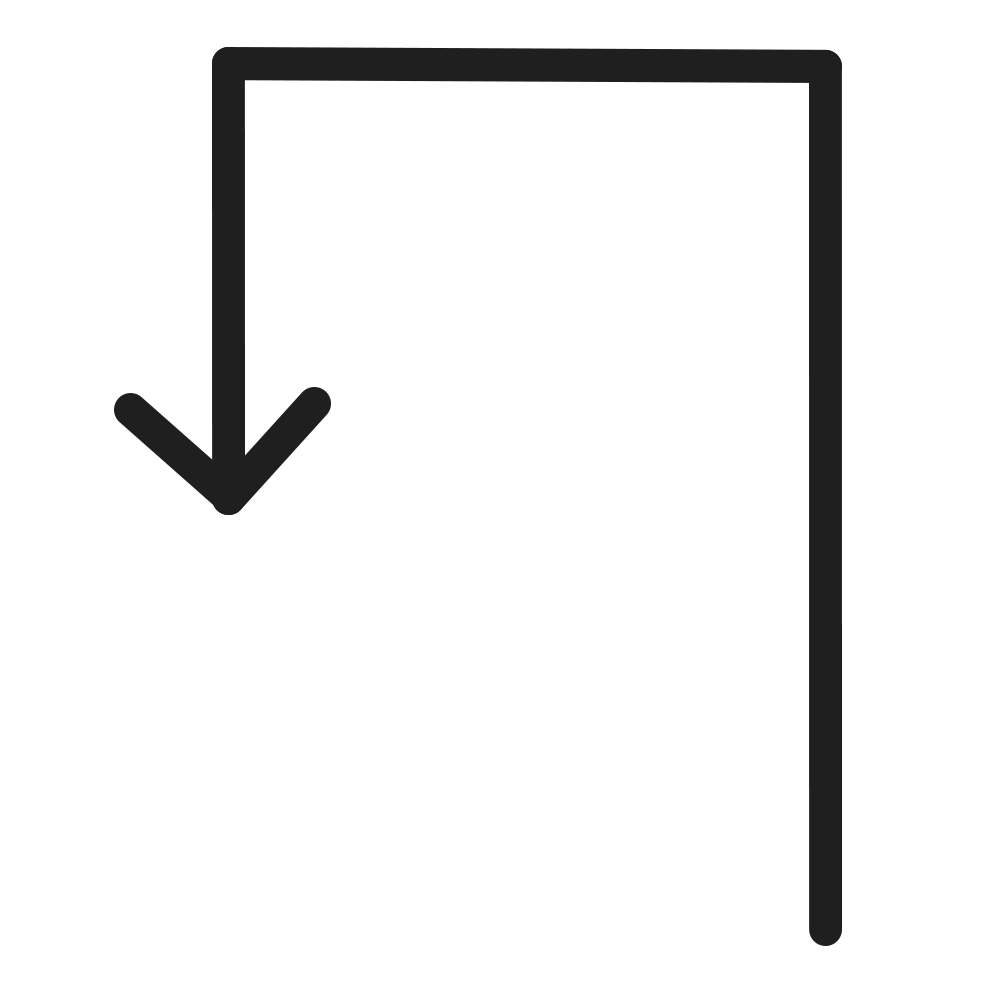
\includegraphics[width=1.1cm]{tablas-images/archi/business/ndti_loop.png}
& R-08 Bucle
& Conductual
& Representa la repetición de una o varias actividades dentro de un proceso hasta que se cumpla una condición determinada.
& Se utiliza exclusivamente dentro de procesos para modelar comportamientos iterativos. \\
\hline


\includegraphics[width=1.1cm]{tablas-images/archi/business/ndti_parallel.png}
& R-09 Paralelización
& Conductual
& Indica la ejecución concurrente de múltiples actividades dentro de un proceso.
& Se emplea para representar bifurcaciones o sincronizaciones de flujos paralelos en procesos. \\
\hline

\end{longtable}

\subsection{Clasificación de relaciones}

\noindent
Las relaciones del lenguaje NDTI se clasifican en:

\begin{itemize}
\item \textbf{Relaciones estructurales:} describen dependencias estáticas entre elementos.
\item \textbf{Relaciones conductuales:} representan interacciones dinámicas y flujos de ejecución.
\end{itemize}

\subsection{Restricciones generales}

\begin{itemize}
\item Las relaciones conductuales solo pueden establecerse entre elementos de comportamiento.
\item Las relaciones estructurales deben mantener coherencia semántica entre los elementos conectados.
\item La relación de especialización solo puede aplicarse entre elementos del mismo tipo conceptual.
\end{itemize}
\newpage


% ==========================================
% CAPÍTULO B: INSTRUMENTOS DE APOYO
% ==========================================
\chapter{Instrumentos y materiales de apoyo}


\phantomsection

% Increment the chapter counter so \thechapter shows the correct number
% and make it referenceable with \ref
\refstepcounter{chapter}

% Manually add this appendix to the Table of Contents
\addcontentsline{toc}{chapter}{Apéndice \thechapter: Búsqueda en bases de datos}

% Add vertical space above the title (mimics standard chapter spacing)
\vspace{40pt}

% Display the actual chapter title (centered, large, bold)
{\centering \normalfont\huge\bfseries Apéndice~\thechapter: Búsqueda en bases de datos~\par}

% Add spacing between title and horizontal rule
\vspace{10pt}

% Draw a horizontal line across the page for visual separation
{\centering \rule{\textwidth}{0.4pt} \par}

% Add vertical space between title section and content
\vspace{40pt}

% Set the running headers for left and right pages
\markboth{Apéndice \thechapter:Búsqueda en bases de datos}{Apéndice \thechapter: Búsqueda en bases de datos}



\FloatBarrier\section{Cadenas de búsqueda}\label{sec:cadenas-busqueda}


\begin{tcolorbox}[
		colback=gray!5,
		colframe=black!60,
		title=Cadena de búsqueda en ACM Full Text Collection para ``Metodología'',
		fonttitle=\bfseries,
		sharp corners=south
	]
	\scriptsize
	\begin{verbatim}
((Abstract:("Notation" OR "Architecture description language" OR "Modeling language") AND Abstract:(“Methodology” OR "Technique" OR "Procedure")) 
OR
(Title:("Notation" OR "Architecture description language" OR "Modeling language") AND Title:(“Methodology” OR "Technique" OR "Procedure")) 
OR
(Keyword:("Notation" OR "Architecture description language" OR "Modeling language") AND Keyword:(“Methodology” OR "Technique" OR "Procedure")))
	\end{verbatim}
\end{tcolorbox}

\begin{tcolorbox}[
		colback=gray!5,
		colframe=black!60,
		title=Cadena de búsqueda en ACM Full Text Collection para ``Tecnología'',
		fonttitle=\bfseries,
		sharp corners=south
	]
	\scriptsize
	\begin{verbatim}
(Abstract:("Notation" OR "Architecture description language" OR "Modeling language") AND Abstract:("Technology" OR "Implementation Information Technology"  OR "Instrument")) 
OR 
(Title:("Notation" OR "Architecture description language" OR "Modeling language") AND Title:("Technology" OR "Implementation Information Technology"  OR "Instrument"))
OR 
(Keyword:("Notation" OR "Architecture description language" OR "Modeling language") AND Keyword:("Technology" OR "Implementation Information Technology" OR "Instrument")) 
	\end{verbatim}
\end{tcolorbox}

\begin{tcolorbox}[
		colback=gray!5,
		colframe=black!60,
		title=Cadena de búsqueda en ACM Full Text Collection para ``Diseño'',
		fonttitle=\bfseries,
		sharp corners=south
	]
	\scriptsize
	\begin{verbatim}
(Abstract:("Notation" OR "Architecture description language" OR "Modeling language") AND Abstract:("Design" OR "Diagram"  OR "Representation")) 
OR 
(Title:("Notation" OR "Architecture description language" OR "Modeling language") AND Title:("Design" OR "Diagram"  OR "Representation")) 
OR 
(Keyword:("Notation" OR "Architecture description language" OR "Modeling language") AND Keyword:("Design" OR "Diagram"  OR "Representation")) 
	\end{verbatim}
\end{tcolorbox}

\begin{tcolorbox}[
		colback=gray!5,
		colframe=black!60,
		title=Cadena de búsqueda en IEEE Xplore para ``Metodología'',
		fonttitle=\bfseries,
		sharp corners=south
	]
	\scriptsize
	\begin{verbatim}
("Abstract":"Notation" OR "Abstract":"Architecture description language" OR "Abstract":"Modeling language") AND ("Abstract":"Technique" OR "Abstract":"Procedure") 
OR 
("Publication Title":"Notation" OR "Publication Title":"Architecture description language" OR "Publication Title":"Modeling language") AND ("Publication Title":"Technique" OR "Publication Title":"Procedure") 
OR 
("Author Keywords":"Notation" OR "Author Keywords":"Architecture description language" OR "Author Keywords":"Modeling language") AND ("Author Keywords":"Technique" OR "Author Keywords":"Procedure")
	\end{verbatim}
\end{tcolorbox}

\begin{tcolorbox}[
		colback=gray!5,
		colframe=black!60,
		title=Cadena de búsqueda en IEEE Xplore para ``Tecnología'',
		fonttitle=\bfseries,
		sharp corners=south
	]
	\scriptsize
	\begin{verbatim}
("Abstract":"Notation" OR "Abstract":"Architecture description language" OR "Abstract":"Modeling language") AND ("Abstract":"Implementation Information Technology" OR "Abstract":"Instrument") 
OR 
("Author Keywords":"Notation" OR "Author Keywords":"Architecture description language" OR "Author Keywords":"Modeling language") AND ("Author Keywords":"Implementation Information Technology" OR "Author Keywords":"Instrument") 
OR 
("Publication Title":"Notation" OR "Publication Title":"Architecture description language" OR "Publication Title":"Modeling language") AND ("Publication Title":"Implementation Information Technology" OR "Publication Title":"Instrument")
	\end{verbatim}
\end{tcolorbox}

\begin{tcolorbox}[
		colback=gray!5,
		colframe=black!60,
		title=Cadena de búsqueda en IEEE Xplore para ``Diseño'',
		fonttitle=\bfseries,
		sharp corners=south
	]
	\scriptsize
	\begin{verbatim}
("Abstract":"Notation" OR "Abstract":"Architecture description language" OR "Abstract":"Modeling language") AND ("Abstract":"Diagram" OR "Abstract":"Representation") 
OR 
("Author Keywords":"Notation" OR "Author Keywords":"Architecture description language" OR "Author Keywords":"Modeling language") AND ("Author Keywords":"Implementation Information Technology" OR "Author Keywords":"Instrument") 
OR 
("Publication Title":"Notation" OR "Publication Title":"Architecture description language" OR "Publication Title":"Modeling language") AND ("Publication Title":"Implementation Information Technology" OR "Publication Title":"Instrument")
	\end{verbatim}
\end{tcolorbox}

\begin{tcolorbox}[
		colback=gray!5,
		colframe=black!60,
		title=Cadena de búsqueda en Springer para ``Metodología'',
		fonttitle=\bfseries,
		sharp corners=south
	]
	\scriptsize
	\begin{verbatim}
(title:("Notation" OR "Architecture description language" OR "Modeling language") AND title:(“Methodology” OR "Technique" OR "Procedure"))
OR
(abstract:("Notation" OR "Architecture description language" OR "Modeling language")AND abstract:(“Methodology” OR "Technique" OR "Procedure"))
OR 
(keyword:("Notation" OR "Architecture description language" OR "Modeling language") AND keyword:(“Methodology” OR "Technique" OR "Procedure"))
	\end{verbatim}
\end{tcolorbox}

\begin{tcolorbox}[
		colback=gray!5,
		colframe=black!60,
		title=Cadena de búsqueda en Springer para ``Tecnología'',
		fonttitle=\bfseries,
		sharp corners=south
	]
	\scriptsize
	\begin{verbatim}
(title:("Notation" OR "Architecture description language" OR "Modeling language") AND title:("Technology" OR "Implementation Information Technology"  OR "Instrument"))
OR
(abstract:("Notation" OR "Architecture description language" OR "Modeling language")AND abstract:("Technology" OR "Implementation Information Technology"  OR "Instrument"))
OR 
(keyword:("Notation" OR "Architecture description language" OR "Modeling language") AND keyword:("Technology" OR "Implementation Information Technology"  OR "Instrument"))
	\end{verbatim}
\end{tcolorbox}

\begin{tcolorbox}[
		colback=gray!5,
		colframe=black!60,
		title=Cadena de búsqueda en Springer para ``Diseño'',
		fonttitle=\bfseries,
		sharp corners=south
	]
	\scriptsize
	\begin{verbatim}
(title:("Notation" OR "Architecture description language" OR "Modeling language") AND title:("Design" OR "Diagram"  OR "Representation")) 
AND
(abstract:("Notation" OR "Architecture description language" OR "Modeling language")AND abstract:("Design" OR "Diagram"  OR "Representation")) 
AND 
(keyword:("Notation" OR "Architecture description language" OR "Modeling language") AND keyword:("Design" OR "Diagram"  OR "Representation")) 
	\end{verbatim}
\end{tcolorbox}

\begin{tcolorbox}[
		colback=gray!5,
		colframe=black!60,
		title=Cadena de búsqueda en ScienceDirect para ``Metodología'',
		fonttitle=\bfseries,
		sharp corners=south
	]
	\scriptsize
	\begin{verbatim}
("Notation" OR "Architecture description language" OR "Modeling language")  AND (“Methodology” OR "Technique" OR "Procedure")
	\end{verbatim}
\end{tcolorbox}

\begin{tcolorbox}[
		colback=gray!5,
		colframe=black!60,
		title=Cadena de búsqueda en ScienceDirect para ``Tecnología'',
		fonttitle=\bfseries,
		sharp corners=south
	]
	\scriptsize
	\begin{verbatim}
("Notation" OR "Architecture description language" OR "Modeling language")  AND ("Technology" OR "Implementation Information Technology"  OR "Instrument")
	\end{verbatim}
\end{tcolorbox}

\begin{tcolorbox}[
		colback=gray!5,
		colframe=black!60,
		title=Cadena de búsqueda en ScienceDirect para ``Diseño'',
		fonttitle=\bfseries,
		sharp corners=south
	]
	\scriptsize
	\begin{verbatim}
("Notation" OR "Architecture description language" OR "Modeling language")  AND ("Design" OR "Diagram"  OR "Representation")
	\end{verbatim}
\end{tcolorbox}

\begin{tcolorbox}[
		colback=gray!5,
		colframe=black!60,
		title=Cadena de búsqueda en Taylor \& Francis para ``Metodología'',
		fonttitle=\bfseries,
		sharp corners=south
	]
	\scriptsize
	\begin{verbatim}
[[Publication Title: "notation"] OR [Publication Title: "architecture description language"] OR [Publication Title: "modeling language"]] AND [[Publication Title: "design"] OR [Publication Title: "diagram"] OR [Publication Title: "representation"]] 
AND 
[[Keywords: "notation"] OR [Keywords: "architecture description language"] OR [Keywords: "modeling language"]] AND [[Keywords: "design"] OR [Keywords: "diagram"] OR [Keywords: "representation"]] 
AND 
[[Abstract: "notation"] OR [Abstract: "architecture description language"] OR [Abstract: "modeling language"]] AND [[Abstract: "design"] OR [Abstract: "diagram"] OR [Abstract: "representation"]]
  \end{verbatim}
\end{tcolorbox}


\begin{tcolorbox}[
		colback=gray!5,
		colframe=black!60,
		title=Cadena de búsqueda en Taylor \& Francis para ``Tecnología'',
		fonttitle=\bfseries,
		sharp corners=south
	]
	\scriptsize
	\begin{verbatim}
[[Publication Title: "notation"] OR [Publication Title: "architecture description language"] OR [Publication Title: "modeling language"]] AND [[Publication Title: "technology"] OR [Publication Title: "implementation information technology"] OR [Publication Title: "instrument"]] 
AND
[[Keywords: "notation"] OR [Keywords: "architecture description language"] OR [Keywords: "modeling language"]] AND [[Keywords: "technology"] OR [Keywords: "implementation information technology"] OR [Keywords: "instrument"]] 
AND
[[Abstract: "notation"] OR [Abstract: "architecture description language"] OR [Abstract: "modeling language"]] AND [[Abstract: "technology"] OR [Abstract: "implementation information technology"] OR [Abstract: "instrument"]]
  \end{verbatim}
\end{tcolorbox}

\begin{tcolorbox}[
		colback=gray!5,
		colframe=black!60,
		title=Cadena de búsqueda en Taylor \& Francis para ``Diseño'',
		fonttitle=\bfseries,
		sharp corners=south
	]
	\scriptsize
	\begin{verbatim}
[[Publication Title: "notation"] OR [Publication Title: "architecture description language"] OR [Publication Title: "modeling language"]] AND [[Publication Title: "design"] OR [Publication Title: "diagram"] OR [Publication Title: "representation"]] 
AND
[[Keywords: "notation"] OR [Keywords: "architecture description language"] OR [Keywords: "modeling language"]] AND [[Keywords: "design"] OR [Keywords: "diagram"] OR [Keywords: "representation"]] 
AND 
[[Abstract: "notation"] OR [Abstract: "architecture description language"] OR [Abstract: "modeling language"]] AND [[Abstract: "design"] OR [Abstract: "diagram"] OR [Abstract: "representation"]]
  \end{verbatim}
\end{tcolorbox}

\section{Búsqueda de artículos sin criterios de inclusión/exclusión}\label{sec:busqueda-sin-criterios}

% ##### Imagenes de busqueda ########

\begin{figure}[H]
	\centering
	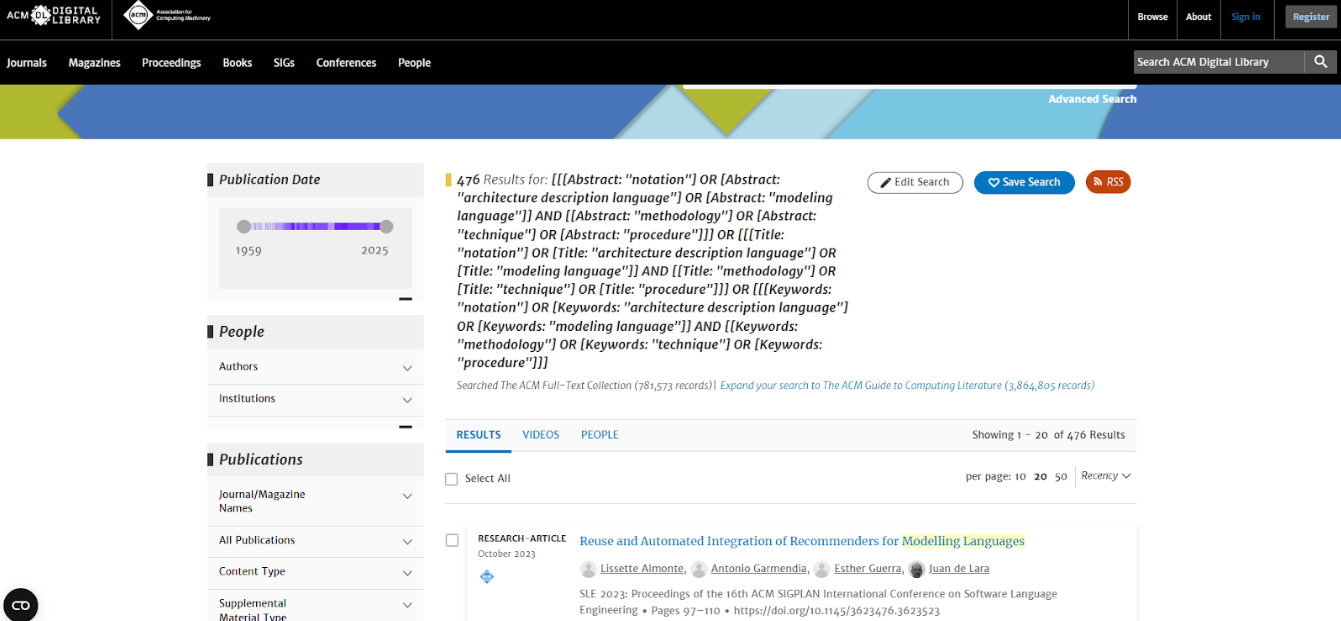
\includegraphics[width=\textwidth,keepaspectratio]{apendices/bases-datos/sin-exclusion/acm.png}
	\caption{Búsqueda de artículos de educación en ACM (Metodología) sin criterios de inclusión/exclusión \\
		Fecha de acceso: 09/04/25 12:38 am
	}\label{fig:busqueda-acm-metodologia-no-exclusion}
\end{figure}

\begin{figure}[H]
	\centering
	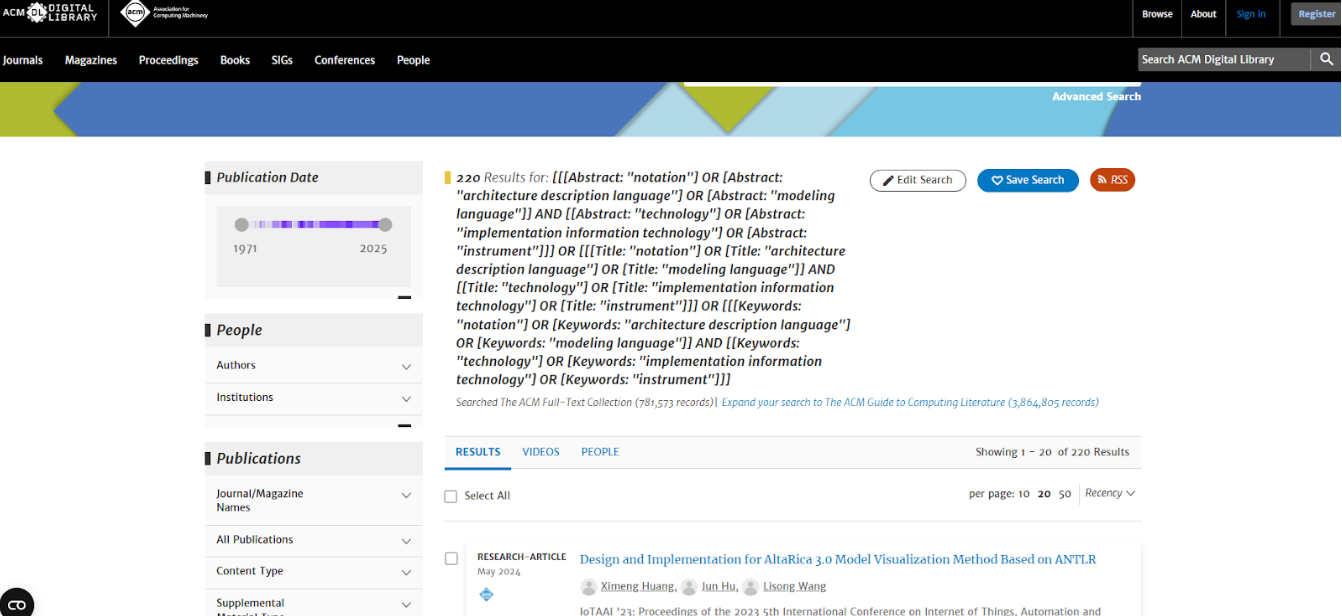
\includegraphics[width=\textwidth,keepaspectratio]{apendices/bases-datos/sin-exclusion/acm2.png}
	\caption{Búsqueda de artículos de educación en ACM (Tecnología) sin criterios de inclusión/exclusión \\
		Fecha de acceso: 09/04/25 12:39 am
	}\label{fig:busqueda-acm-tecnologia-no-exclusion}
\end{figure}

\begin{figure}[H]
	\centering
	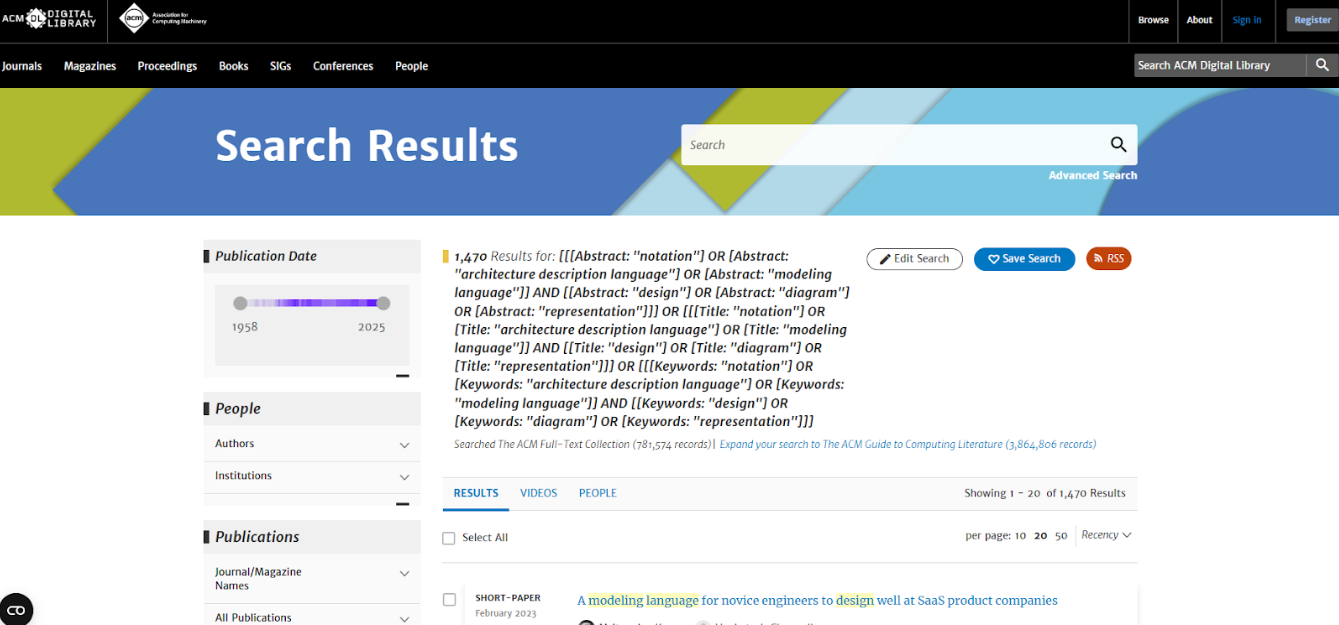
\includegraphics[width=\textwidth,keepaspectratio]{apendices/bases-datos/sin-exclusion/acm3.png}
	\caption{Búsqueda de artículos de educación en ACM (Diseño) sin criterios de inclusión/exclusión \\
		Fecha de acceso: 09/04/25 12:40 am
	}\label{fig:busqueda-acm-diseno-no-exclusion}
\end{figure}

\FloatBarrier

\begin{figure}[H]
	\centering
	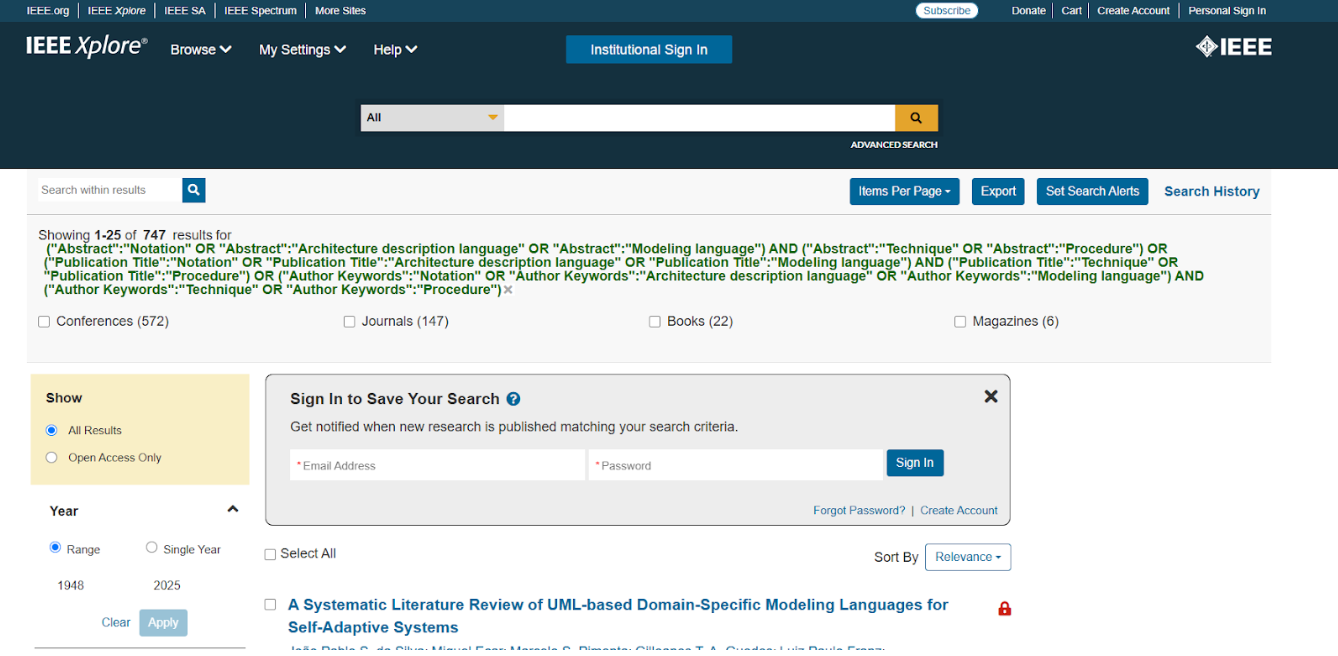
\includegraphics[width=\textwidth,keepaspectratio]{apendices/bases-datos/sin-exclusion/ieee.png}
	\caption{Búsqueda de artículos de educación en IEEE Xplore (Metodología) sin criterios de inclusión/exclusión \\
		Fecha de acceso: 09/04/25 12:47 am
	}\label{fig:busqueda-ieee-metodologia-no-exclusion}
\end{figure}

\begin{figure}[H]
	\centering
	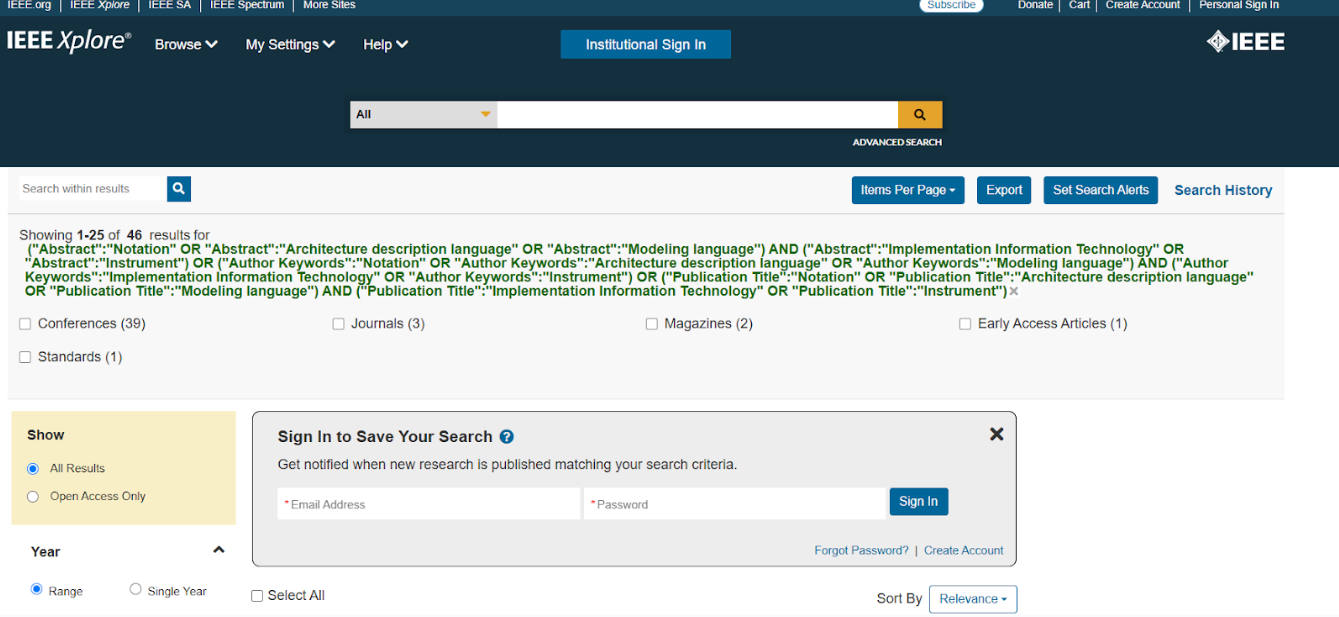
\includegraphics[width=\textwidth,keepaspectratio]{apendices/bases-datos/sin-exclusion/ieee2.png}
	\caption{Búsqueda de artículos de educación en IEEE Xplore (Tecnología) sin criterios de inclusión/exclusión \\
		Fecha de acceso: 09/04/25 12:53 am
	}\label{fig:busqueda-ieee-tecnologia-no-exclusion}

\begin{figure}[H]
	\centering
	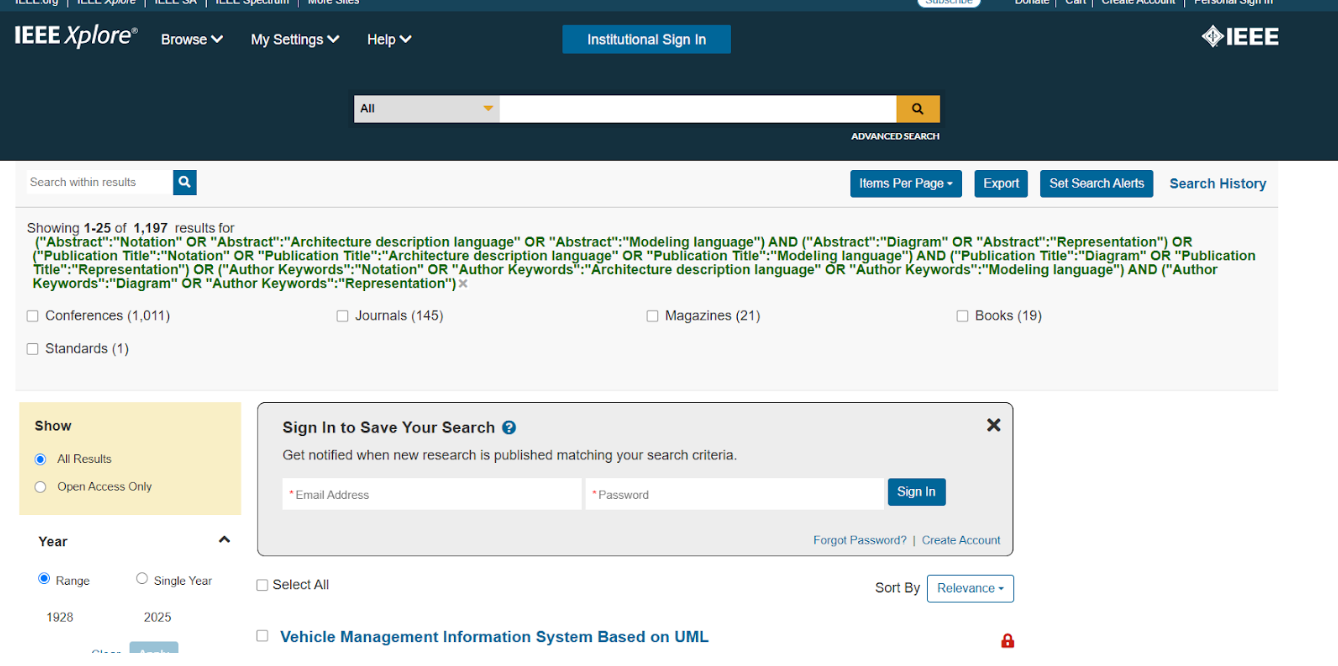
\includegraphics[width=\textwidth,keepaspectratio]{apendices/bases-datos/sin-exclusion/ieee3.png}
	\caption{Búsqueda de artículos de educación en IEEE Xplore (Diseño) sin criterios de inclusión/exclusión \\
		Fecha de acceso: 09/04/25 12:56 am
	}\label{fig:busqueda-ieee-diseno-no-exclusion}

\end{figure}

\FloatBarrier

\begin{figure}[H]
	\centering
	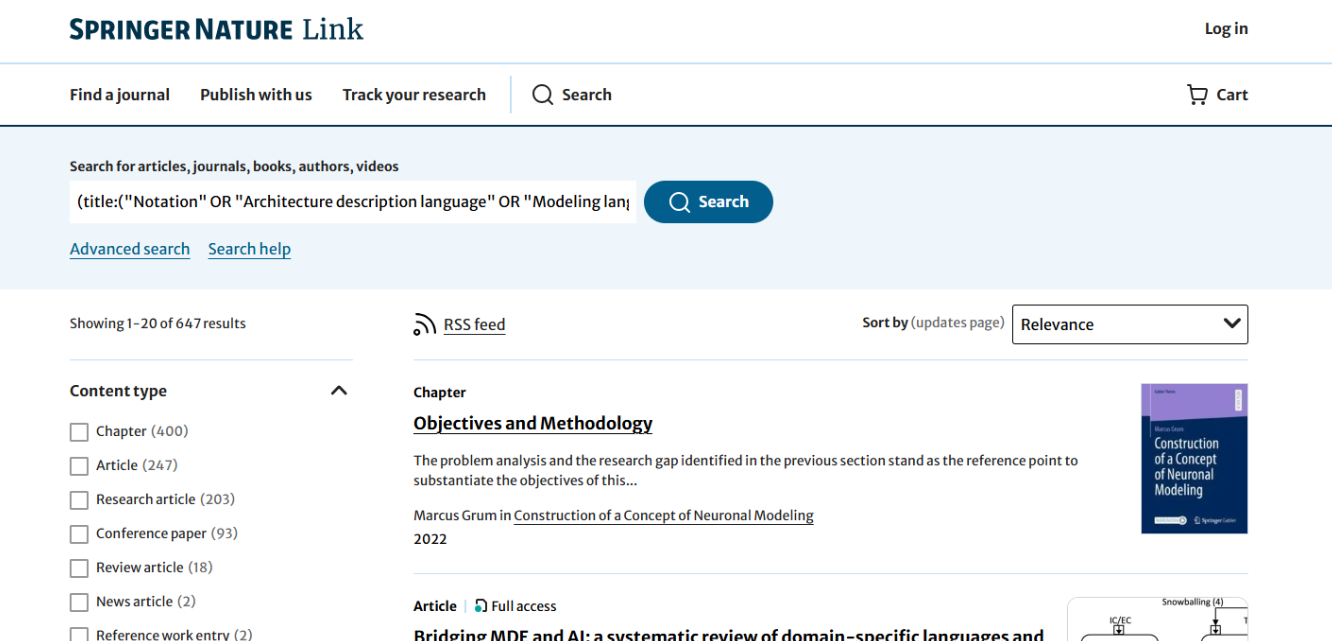
\includegraphics[width=\textwidth,keepaspectratio]{apendices/bases-datos/sin-exclusion/springer.png}
	\caption{Búsqueda de artículos de investigación en Springer Nature (Metodología) sin criterios de inclusión/exclusión \\
		Fecha de acceso: 09/04/25 02:15 pm
	}\label{fig:busqueda-springer-metodologia-no-exclusion}
\end{figure}

\begin{figure}[H]
	\centering
	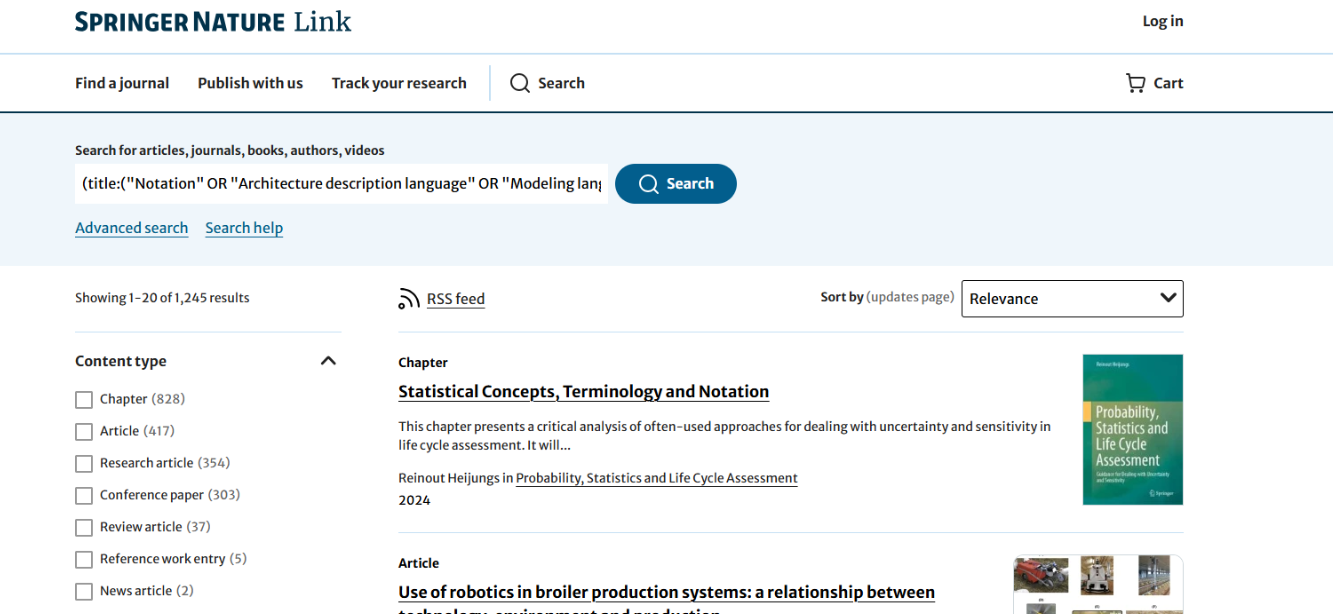
\includegraphics[width=\textwidth,keepaspectratio]{apendices/bases-datos/sin-exclusion/springer2.png}
	\caption{Búsqueda de artículos de investigación en Springer Nature (Tecnología) sin criterios de inclusión/exclusión \\
		Fecha de acceso: 09/04/25 02:16 pm
	}\label{fig:busqueda-springer-tecnologia-no-exclusion}
\end{figure}

\begin{figure}[H]
	\centering
	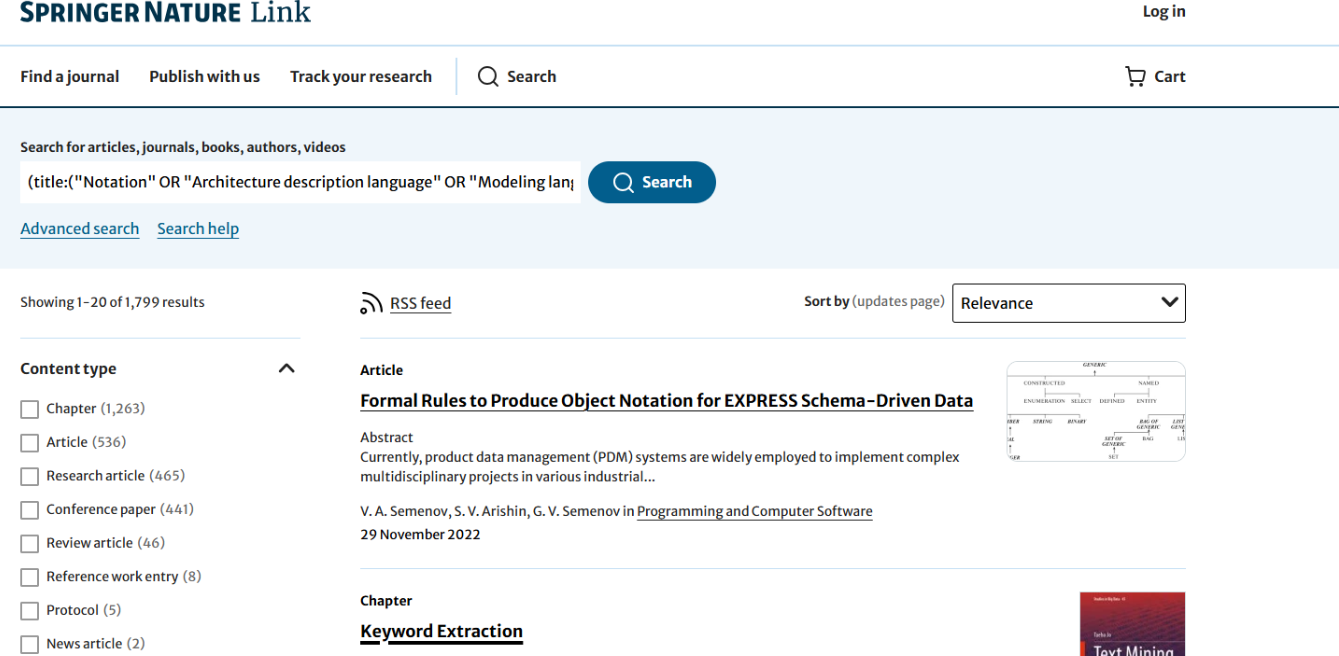
\includegraphics[width=\textwidth,keepaspectratio]{apendices/bases-datos/sin-exclusion/springer3.png}
	\caption{Búsqueda de artículos de investigación en Springer Nature (Diseño) sin criterios de inclusión/exclusión \\
		Fecha de acceso: 09/04/25 02:17 pm
	}\label{fig:busqueda-springer-diseno-no-exclusion}
\end{figure}

\FloatBarrier

\begin{figure}[H]
	\centering
	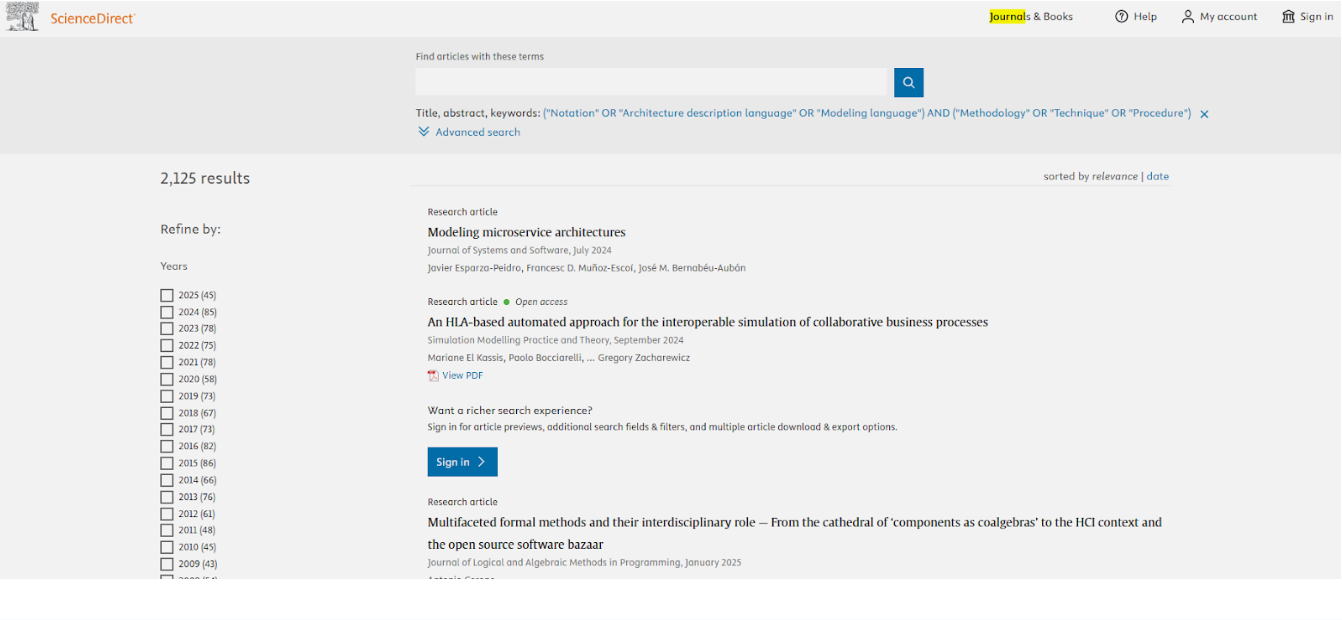
\includegraphics[width=\textwidth,keepaspectratio]{apendices/bases-datos/sin-exclusion/science-direct.png}
	\caption{Búsqueda de artículos de investigación en ScienceDirect (Metodología) sin criterios de inclusión/exclusión \\
		Fecha de acceso: 09/04/25 01:32 am
	}\label{fig:busqueda-science-direct-metodologia-no-exclusion}
\end{figure}

\begin{figure}[H]
	\centering
	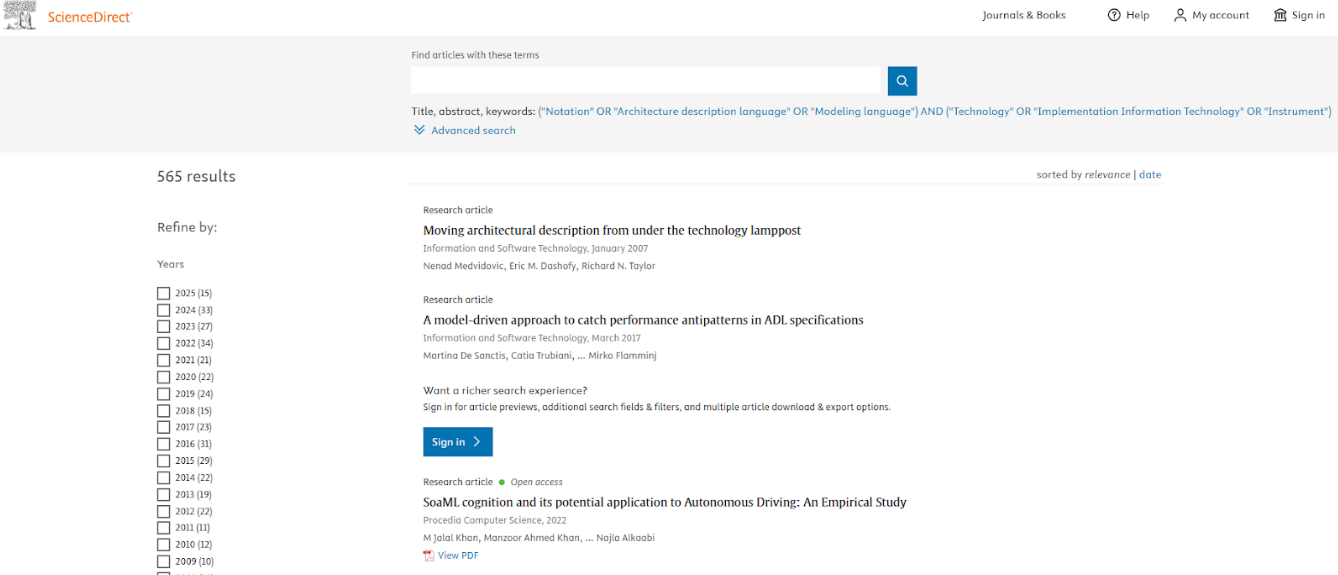
\includegraphics[width=\textwidth,keepaspectratio]{apendices/bases-datos/sin-exclusion/science-direct2.png}
	\caption{Búsqueda de artículos de investigación en ScienceDirect (Tecnología) sin criterios de inclusión/exclusión \\
		Fecha de acceso: 09/04/25 01:36 am
	}\label{fig:busqueda-science-direct-tecnologia-no-exclusion}
\end{figure}

\begin{figure}[H]
	\centering
	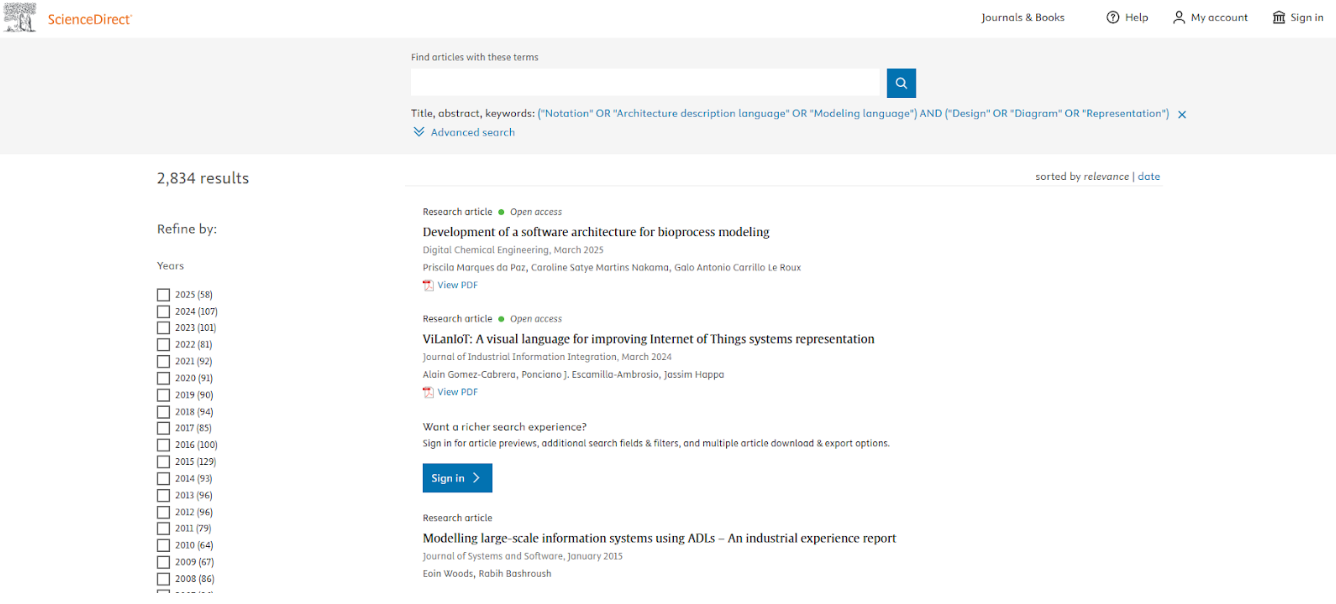
\includegraphics[width=\textwidth,keepaspectratio]{apendices/bases-datos/sin-exclusion/science-direct3.png}
	\caption{Búsqueda de artículos de investigación en ScienceDirect (Diseño) sin criterios de inclusión/exclusión \\
		Fecha de acceso: 09/04/25 01:37 am
	}\label{fig:busqueda-science-direct-diseno-no-exclusion}
\end{figure}

\FloatBarrier

\begin{figure}[H]
	\centering
	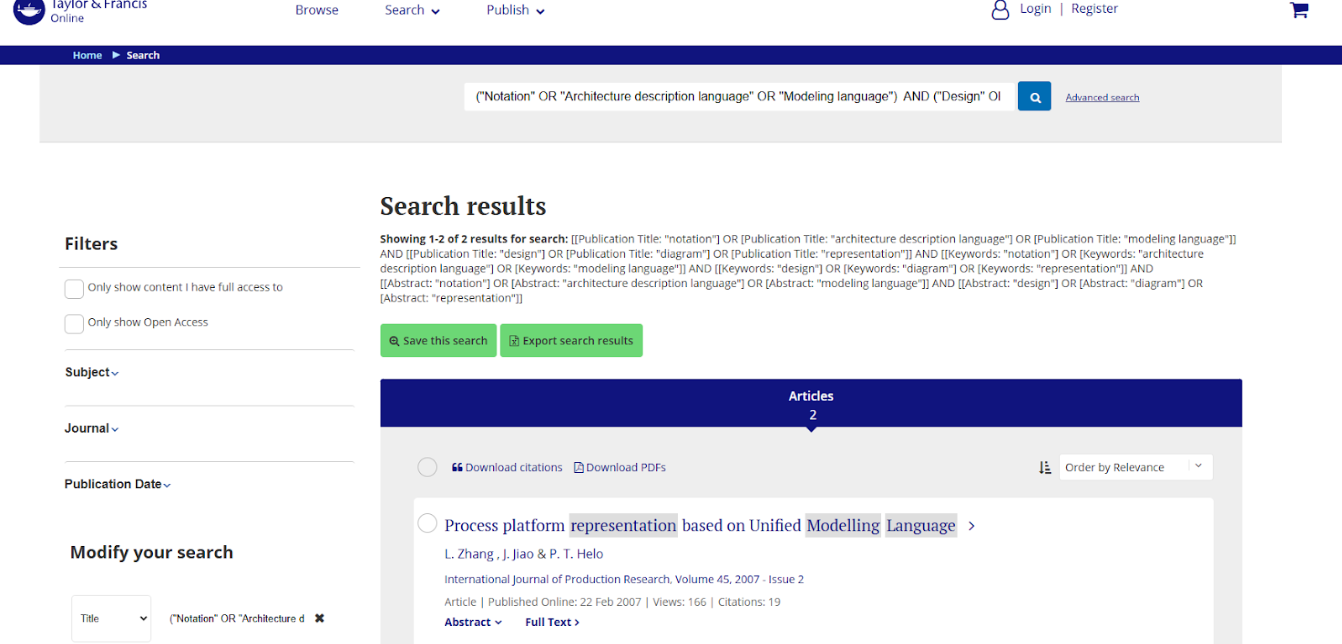
\includegraphics[width=\textwidth,keepaspectratio]{apendices/bases-datos/sin-exclusion/TyF.png}
	\caption{Búsqueda de artículos de investigación en Taylor & Francis (Metodología) sin criterios de inclusión/exclusión \\
		Fecha de acceso: 09/04/25 02:32 pm
	}\label{fig:busqueda-taylor-and-francis-direct-metodologia-no-exclusion}
\end{figure}

\begin{figure}[H]
	\centering
	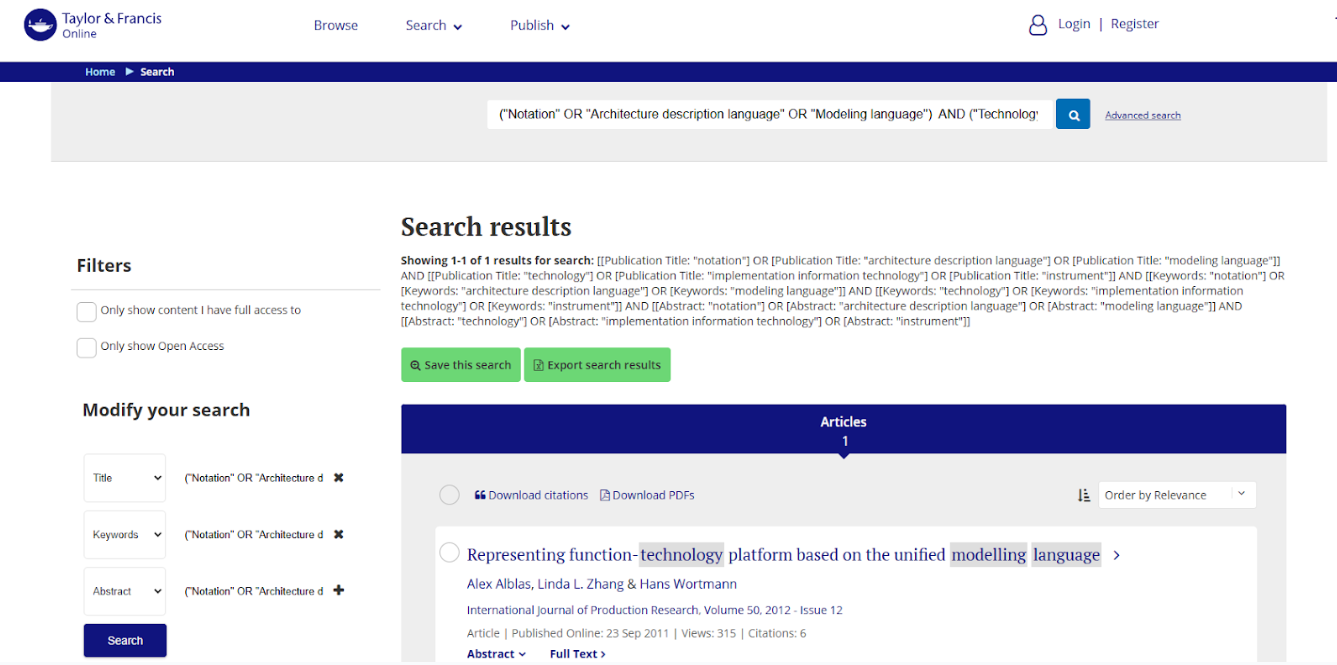
\includegraphics[width=\textwidth,keepaspectratio]{apendices/bases-datos/sin-exclusion/TyF2.png}
	\caption{Búsqueda de artículos de investigación en Taylor & Francis (Tecnología) sin criterios de inclusión/exclusión \\
		Fecha de acceso: 09/04/25 02:35 pm
	}\label{fig:busqueda-taylor-and-francis-direct-tecnologia-no-exclusion}
\end{figure}

\begin{figure}[H]
	\centering
	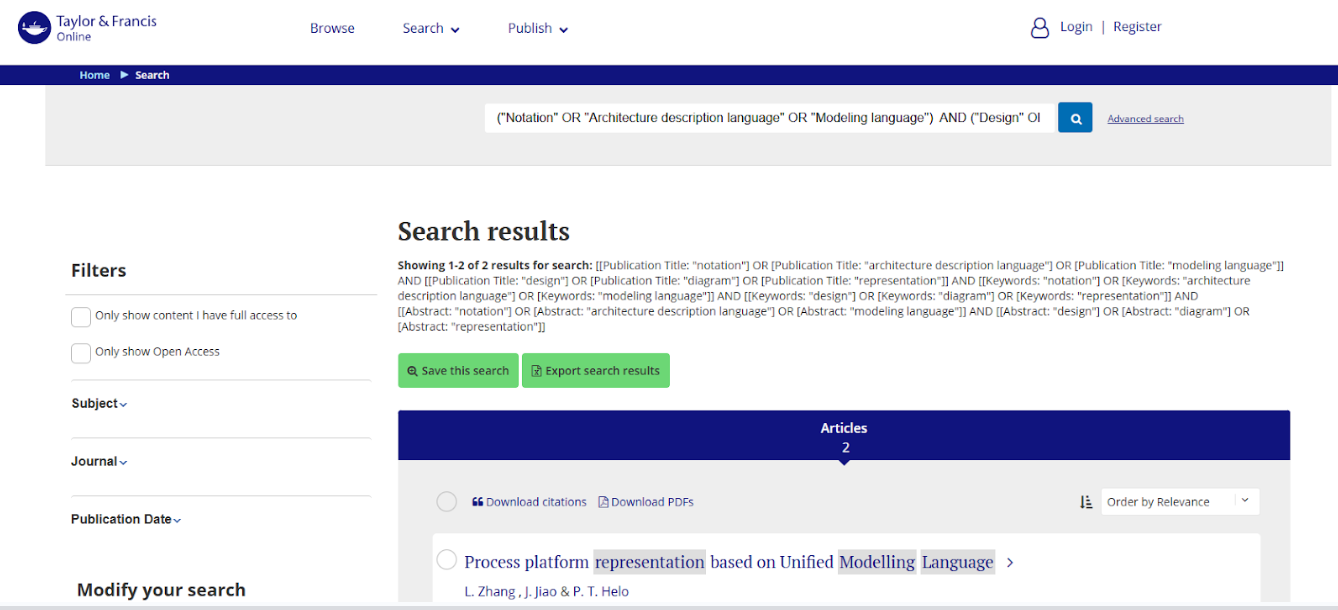
\includegraphics[width=\textwidth,keepaspectratio]{apendices/bases-datos/sin-exclusion/TyF3.png}
	\caption{Búsqueda de artículos de investigación en Taylor & Francis (Diseño) sin criterios de inclusión/exclusión \\
		Fecha de acceso: 09/04/25 02:37 pm
	}\label{fig:busqueda-taylor-and-francis-direct-diseno-no-exclusion}
\end{figure}


%########## Fin Imagenes %###################


\section{Búsqueda de artículos con criterios de inclusión/exclusión}\label{sec:busqueda-con-criterios}

\begin{figure}[H]
	\centering
	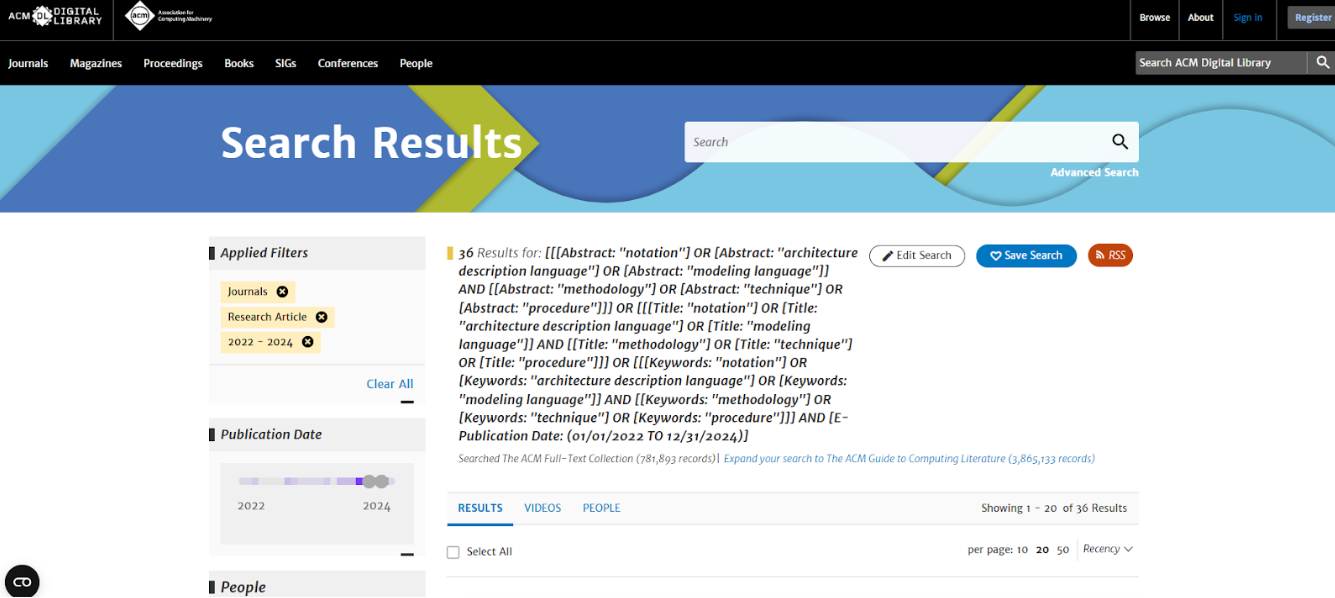
\includegraphics[width=\textwidth,keepaspectratio]{apendices/bases-datos/con-exclusion/acm.png}
	\caption{Búsqueda de artículos de educación en ACM (Metodología) con criterios de inclusión/exclusión \\
		Fecha de acceso: 09/04/25 02:37 pm
	}\label{fig:busqueda-acm-metodologia-con-exclusion}
\end{figure}

\begin{figure}[H]
	\centering
	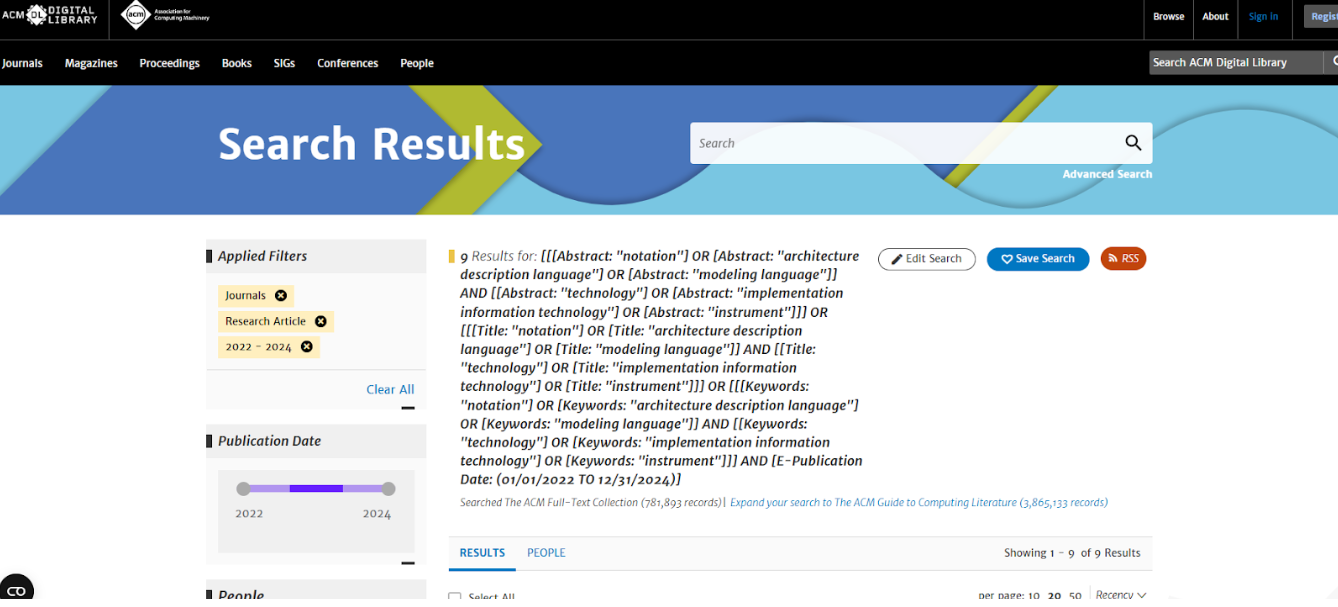
\includegraphics[width=\textwidth,keepaspectratio]{apendices/bases-datos/con-exclusion/acm2.png}
	\caption{Búsqueda de artículos de educación en ACM (Tecnología) con criterios de inclusión/exclusión \\
		Fecha de acceso: 09/04/25 03:27 pm
	}\label{fig:busqueda-acm-tecnologia-con-exclusion}
\end{figure}

\begin{figure}[H]
	\centering
	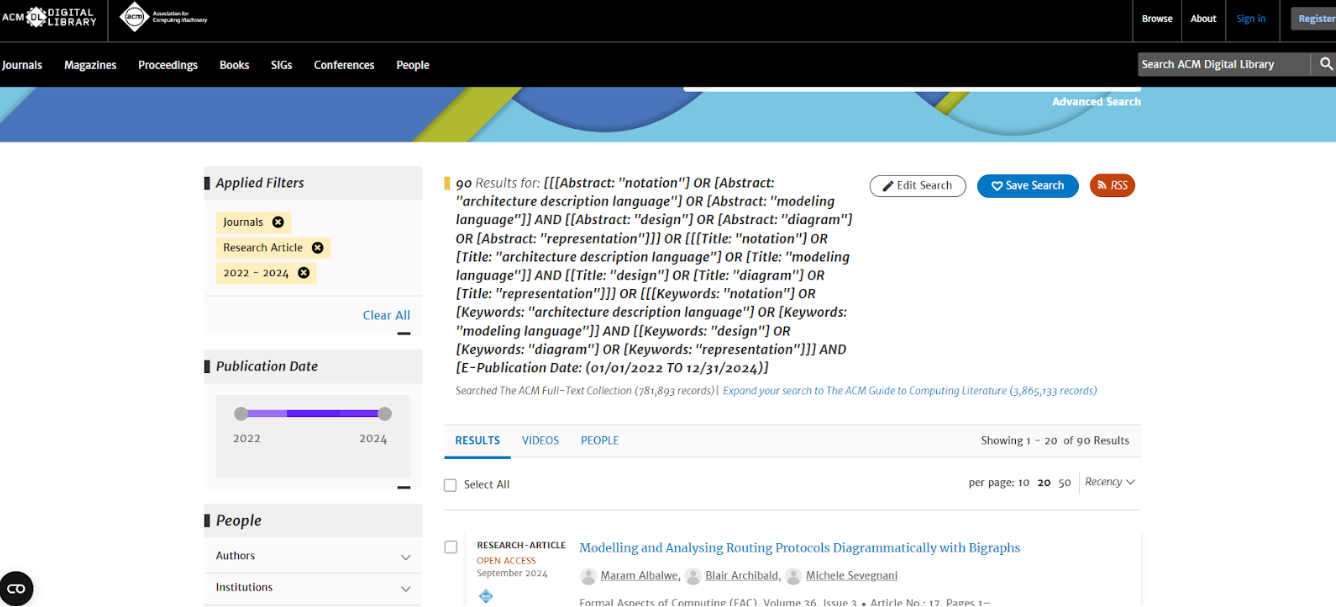
\includegraphics[width=\textwidth,keepaspectratio]{apendices/bases-datos/con-exclusion/acm3.png}
	\caption{Búsqueda de artículos de educación en ACM (Diseño) con criterios de inclusión/exclusión \\
		Fecha de acceso: 09/04/25 03:29 pm
	}\label{fig:busqueda-acm-diseno-con-exclusion}
\end{figure}

\FloatBarrier

\begin{figure}[H]
	\centering
	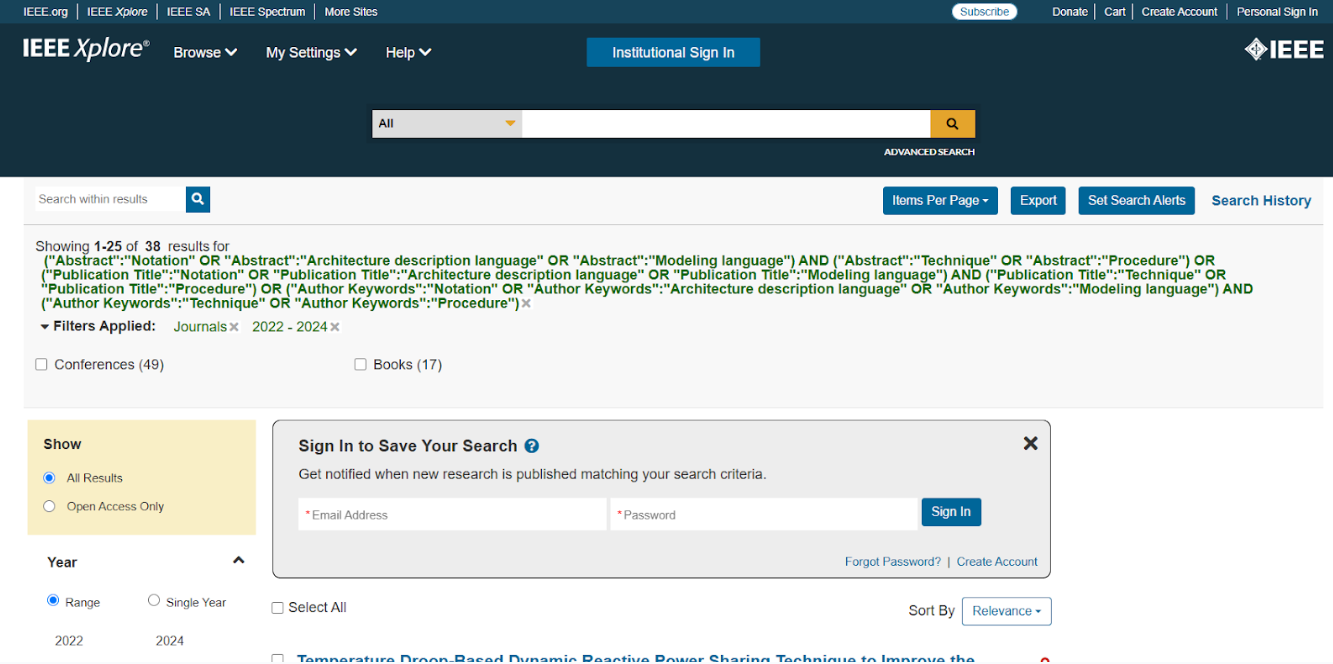
\includegraphics[width=\textwidth,keepaspectratio]{apendices/bases-datos/con-exclusion/ieee.png}
	\caption{Búsqueda de artículos de educación en IEEE Xplore (Metodología) con criterios de inclusión/exclusión \\
		Fecha de acceso: 09/04/25 03:31 pm
	}\label{fig:busqueda-ieee-metodologia-con-exclusion}
\end{figure}

\begin{figure}[H]
	\centering
	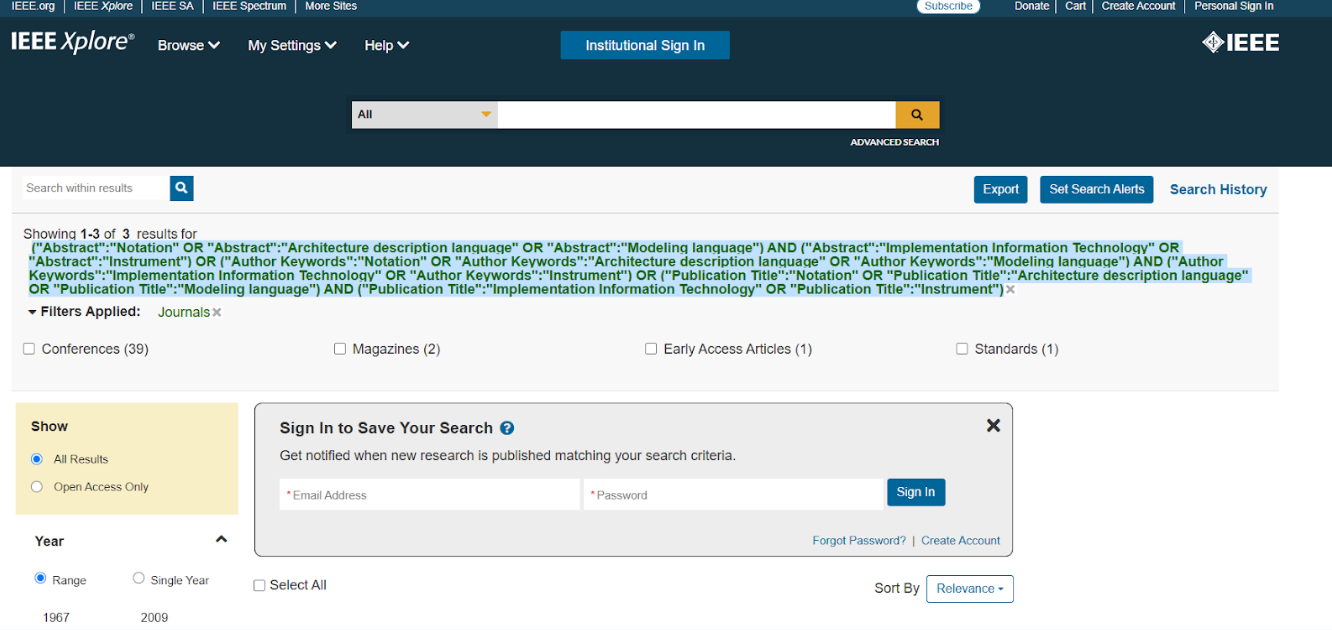
\includegraphics[width=\textwidth,keepaspectratio]{apendices/bases-datos/con-exclusion/ieee2.png}
	\caption{Búsqueda de artículos de educación en IEEE Xplore (Tecnología) con criterios de inclusión/exclusión \\
		Fecha de acceso: 09/04/25 03:35 pm
	}\label{fig:busqueda-ieee-tecnologia-con-exclusion}
\end{figure}

\begin{figure}[H]
	\centering
	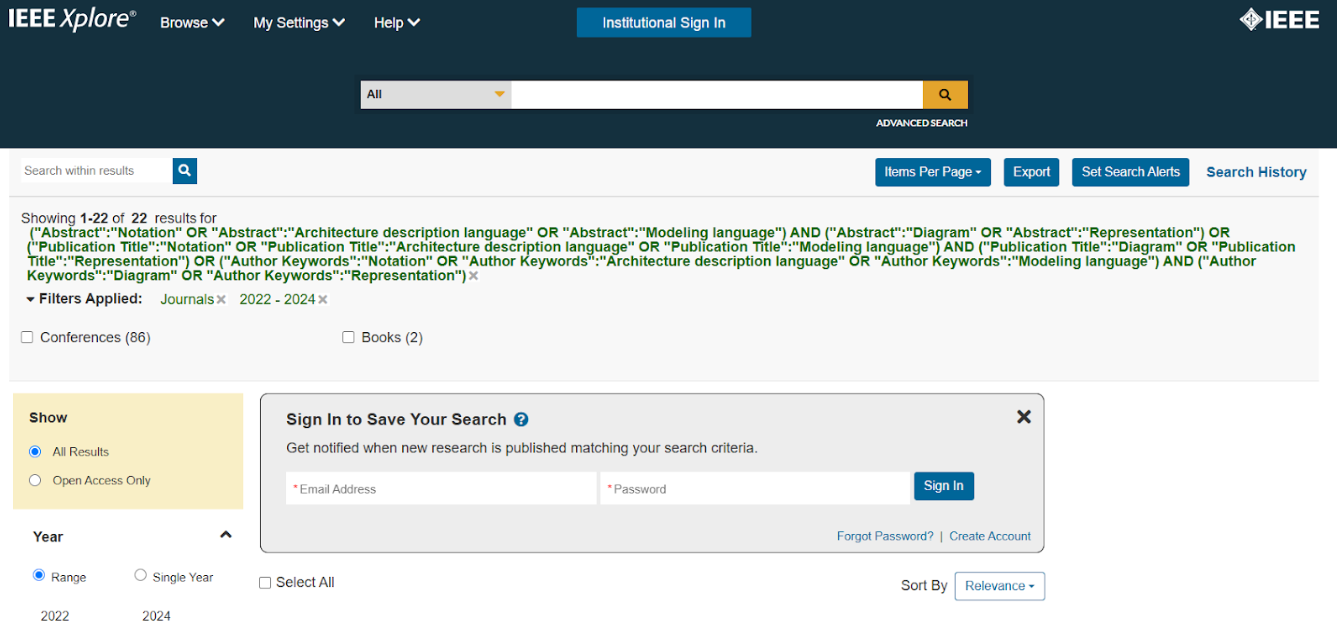
\includegraphics[width=\textwidth,keepaspectratio]{apendices/bases-datos/con-exclusion/ieee3.png}
	\caption{Búsqueda de artículos de educación en IEEE Xplore (Diseño) con criterios de inclusión/exclusión \\
		Fecha de acceso: 09/04/25 03:38 pm
	}\label{fig:busqueda-ieee-diseno-con-exclusion}
\end{figure}

\FloatBarrier

\begin{figure}[H]
	\centering
	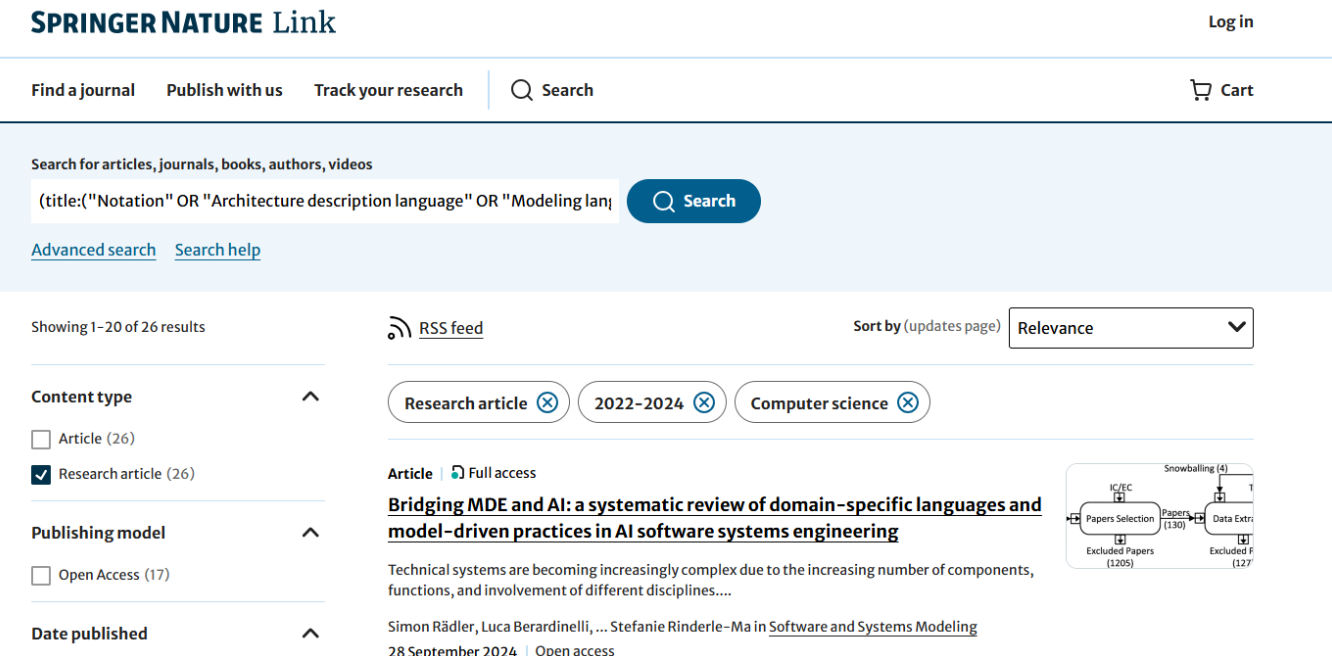
\includegraphics[width=\textwidth,keepaspectratio]{apendices/bases-datos/con-exclusion/springer.png}
	\caption{Búsqueda de artículos de investigación en Springer Nature (Metodología) sin criterios de inclusión/exclusión \\
		Fecha de acceso: 09/04/25 05:52 pm
	}\label{fig:busqueda-springer-metodologia-con-exclusion}
\end{figure}

\begin{figure}[H]
	\centering
	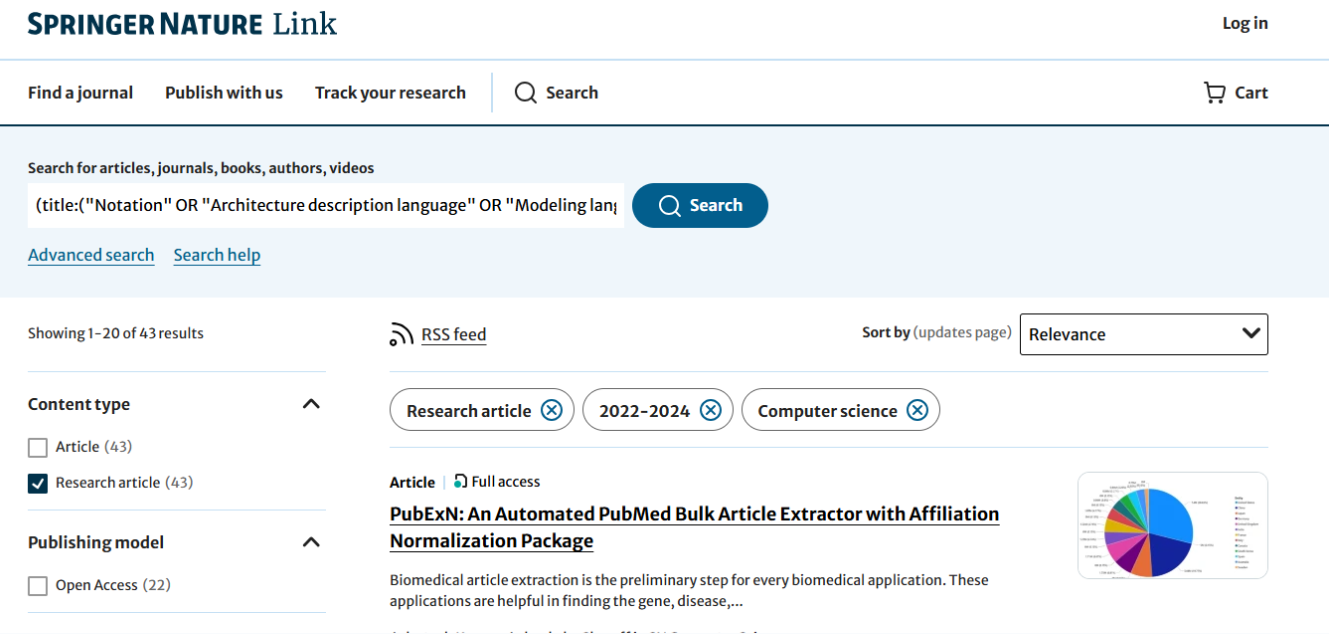
\includegraphics[width=\textwidth,keepaspectratio]{apendices/bases-datos/con-exclusion/springer2.png}
	\caption{Búsqueda de artículos de investigación en Springer Nature (Tecnología) sin criterios de inclusión/exclusión \\
		Fecha de acceso: 09/04/25 05:54 pm
	}\label{fig:busqueda-springer-tecnologia-con-exclusion}
\end{figure}

\begin{figure}[H]
	\centering
	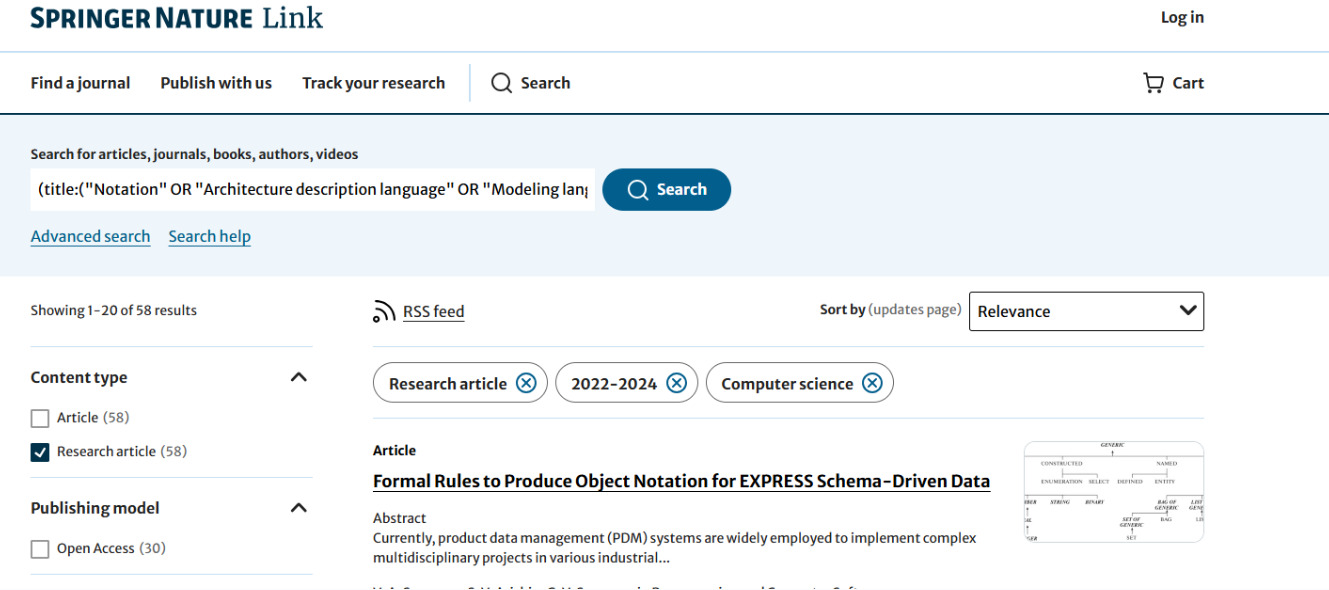
\includegraphics[width=\textwidth,keepaspectratio]{apendices/bases-datos/con-exclusion/springer3.png}
	\caption{Búsqueda de artículos de investigación en Springer Nature (Diseño) sin criterios de inclusión/exclusión \\
		Fecha de acceso: 09/04/25 05:57 pm
	}\label{fig:busqueda-springer-diseno-con-exclusion}
\end{figure}

\FloatBarrier

\begin{figure}[H]
	\centering
	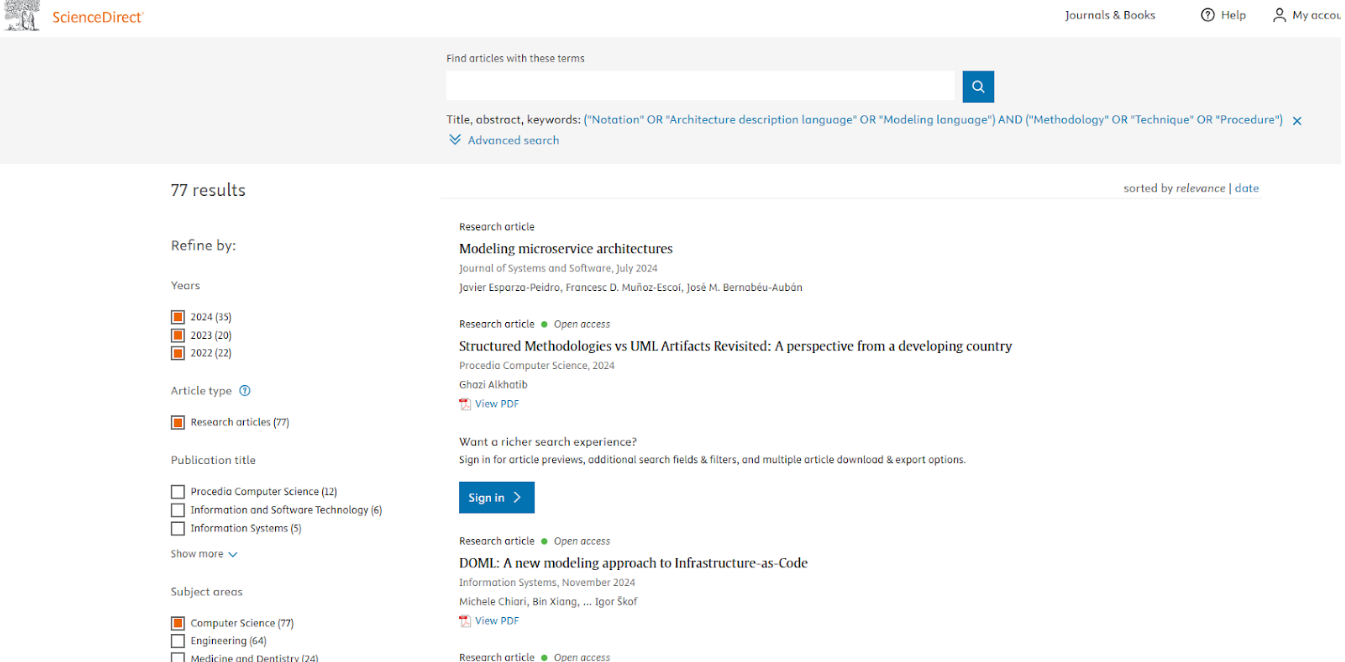
\includegraphics[width=\textwidth,keepaspectratio]{apendices/bases-datos/con-exclusion/science-direct.png}
	\caption{Búsqueda de artículos de investigación en Science Direct (Metodología) sin criterios de inclusión/exclusión \\
		Fecha de acceso: 09/04/25 05:57 pm
	}\label{fig:busqueda-science-direct-metodologia-con-exclusion}
\end{figure}

\begin{figure}[H]
	\centering
	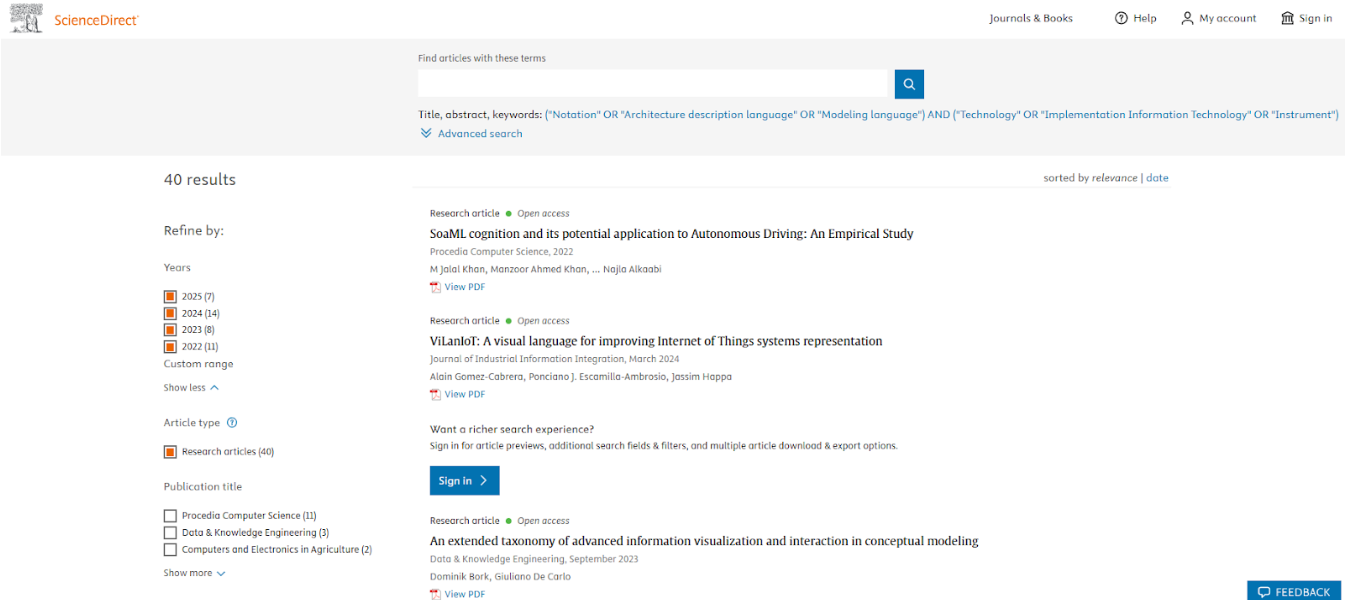
\includegraphics[width=\textwidth,keepaspectratio]{apendices/bases-datos/con-exclusion/science-direct2.png}
	\caption{Búsqueda de artículos de investigación en Science Direct (Tecnología) sin criterios de inclusión/exclusión \\
		Fecha de acceso: 09/04/25 06:02 pm
	}\label{fig:busqueda-science-direct-technologia-con-exclusion}
\end{figure}

\begin{figure}[H]
	\centering
	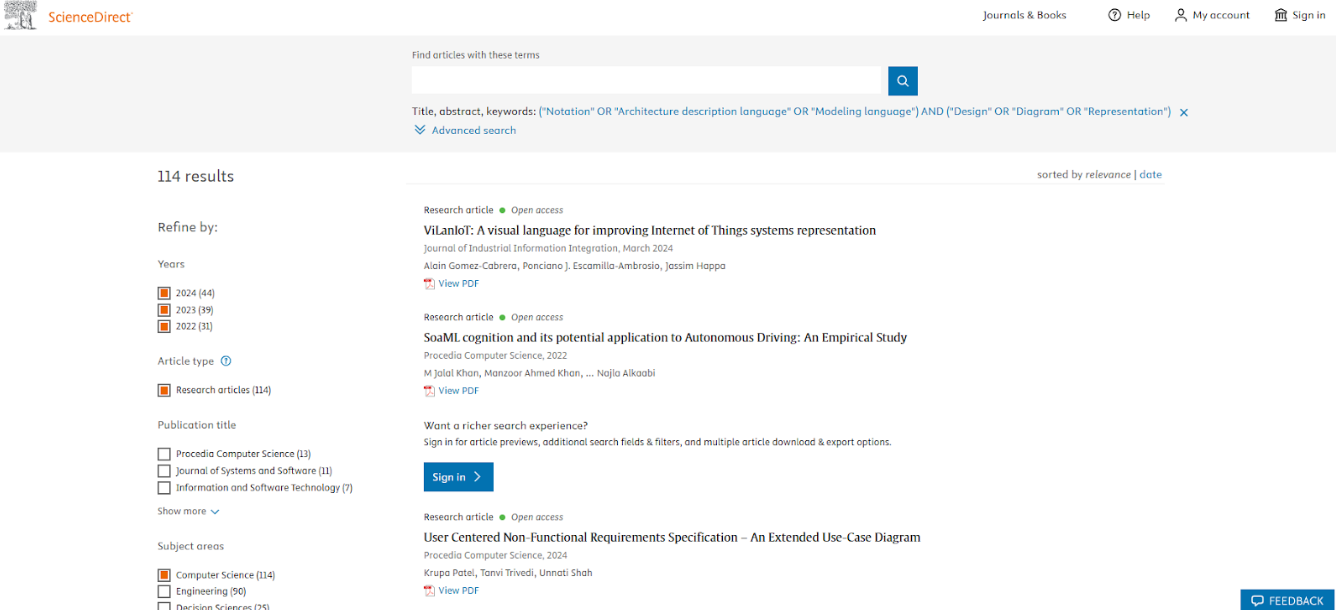
\includegraphics[width=\textwidth,keepaspectratio]{apendices/bases-datos/con-exclusion/science-direct3.png}
	\caption{Búsqueda de artículos de investigación en Science Direct (Diseño) sin criterios de inclusión/exclusión \\
		Fecha de acceso: 09/04/25 06:03 pm
	}\label{fig:busqueda-science-direct-diseno-con-exclusion}
\end{figure}

\FloatBarrier

\begin{figure}[H]
	\centering
	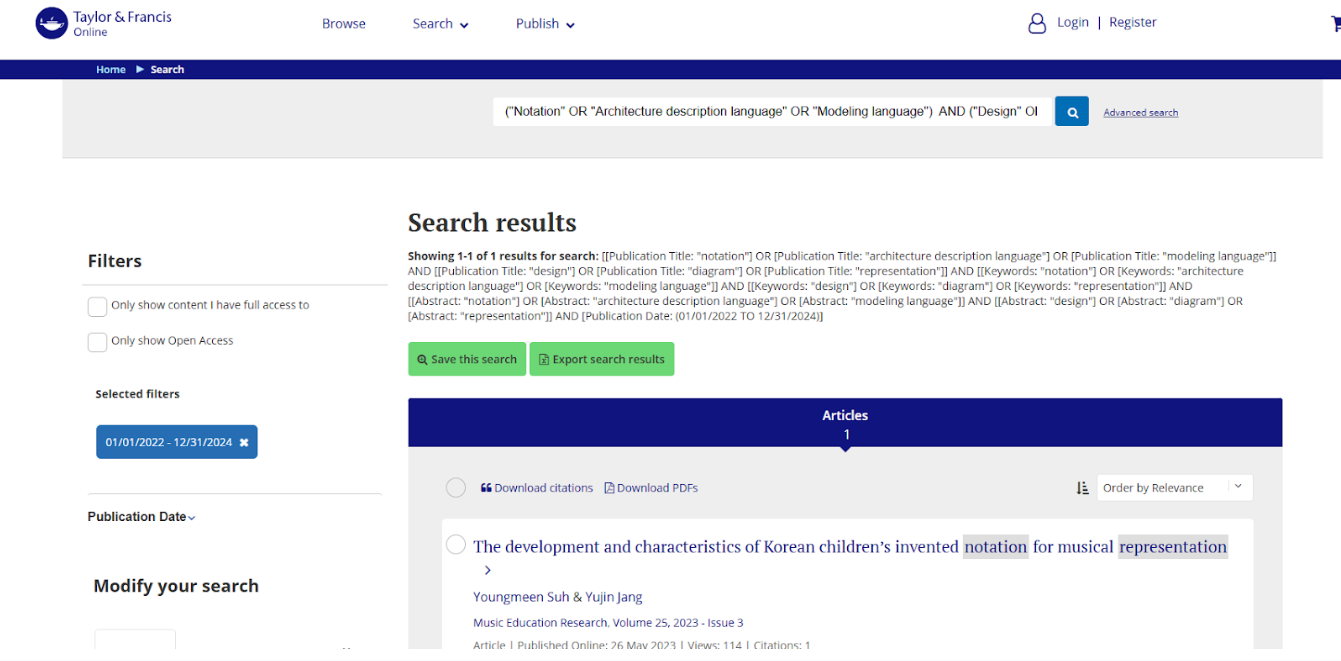
\includegraphics[width=\textwidth,keepaspectratio]{apendices/bases-datos/con-exclusion/TyF.png}
	\caption{Búsqueda de artículos de investigación en Taylor & Francis (Metodología) sin criterios de inclusión/exclusión \\
		Fecha de acceso: 09/04/25 06:13 pm
	}\label{fig:busqueda-taylor-and-francis-metodologia-con-exclusion}
\end{figure}

\begin{figure}[H]
	\centering
	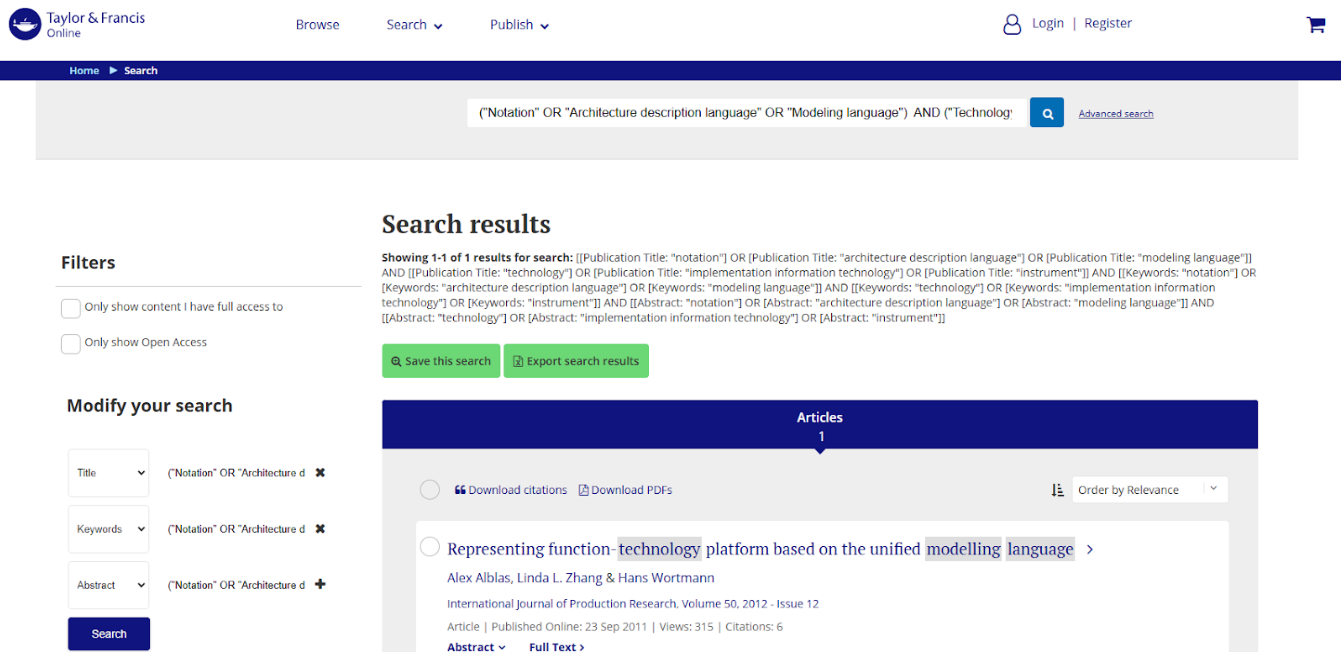
\includegraphics[width=\textwidth,keepaspectratio]{apendices/bases-datos/con-exclusion/TyF2.png}
	\caption{Búsqueda de artículos de investigación en Taylor & Francis (Tecnología) sin criterios de inclusión/exclusión \\
		Fecha de acceso: 09/04/25 06:17 pm
	}\label{fig:busqueda-taylor-and-francis-tecnologia-con-exclusion}
\end{figure}

\begin{figure}[H]
	\centering
	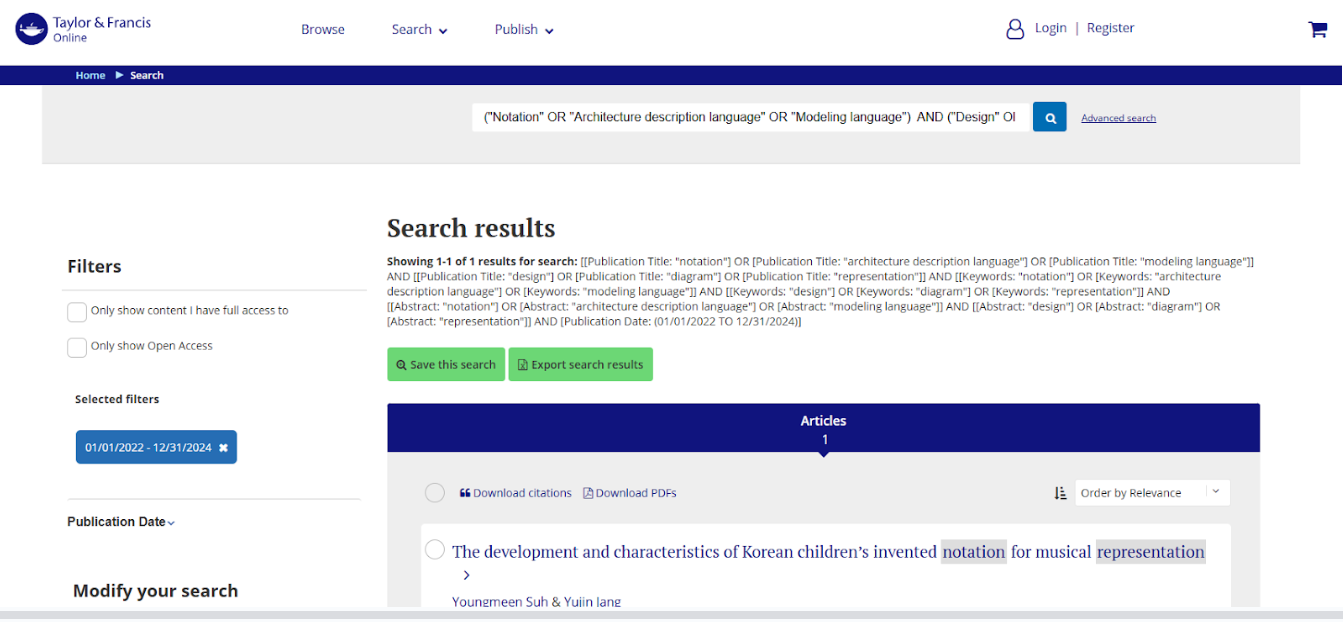
\includegraphics[width=\textwidth,keepaspectratio]{apendices/bases-datos/con-exclusion/TyF3.png}
	\caption{Búsqueda de artículos de investigación en Taylor & Francis (Diseño) sin criterios de inclusión/exclusión \\
		Fecha de acceso: 09/04/25 06:18 pm
	}\label{fig:busqueda-taylor-and-francis-diseno-con-exclusion}
\end{figure}
\newpage

\phantomsection

% Increment the chapter counter so \thechapter shows the correct number
% and make it referenceable with \ref
\refstepcounter{chapter}
\label{chap:plantilla-dar}


% Manually add this appendix to the Table of Contents
\addcontentsline{toc}{chapter}{Apéndice \thechapter: Plantilla análisis DAR}

% Add vertical space above the title (mimics standard chapter spacing)
\vspace{40pt}

% Display the actual chapter title (centered, large, bold)
{\centering \normalfont\huge\bfseries Apéndice~\thechapter: Plantilla análisis DAR~\par}

% Add spacing between title and horizontal rule
\vspace{10pt}

% Draw a horizontal line across the page for visual separation
{\centering \rule{\textwidth}{0.4pt} \par}

% Add vertical space between title section and content
\vspace{40pt}

% Set the running headers for left and right pages
\markboth{Apéndice \thechapter: Plantilla análisis DAR}{Apéndice \thechapter: Plantilla análisis DAR}



\begin{table}[H]
	\centering
	\renewcommand{\arraystretch}{1.2}
	\fontsize{9pt}{10pt}\selectfont
	\caption{Plantilla análisis \DAR.}
	\label{tab:plantilla-analisis_dar}
	
	\resizebox{\textwidth}{!}{
	\begin{tabular}{|c|c|c|c|c|c|c|}
		\hline
		\textbf{Notación} & \textbf{Popularidad} & \textbf{Documentación} & \textbf{Apalancamiento y Formalidad} & \textbf{Vigencia} & \textbf{Minimalismo} & \textbf{Promedio} \\
		\hline
		\multicolumn{1}{|c|}{\textbf{Conjunto}} & \multicolumn{5}{c|}{\textbf{Puntaje}} & \\
		\hline
		Vanilla   &  &  &  &  &  &  \\
		\hline
		Grid      &  &  &  &  &  &  \\
		\hline
		Java      &  &  &  &  &  &  \\
		\hline
		Scheduler &  &  &  &  &  &  \\
		\hline
		Local     &  &  &  &  &  &  \\
		\hline
		Parallel  &  &  &  &  &  &  \\
		\hline
		VM        &  &  &  &  &  &  \\
		\hline
		Container &  &  &  &  &  &  \\
		\hline
		Docker    &  &  &  &  &  &  \\
		\hline
	\end{tabular}
	}
\end{table}

\newpage

% ==========================================
% CAPÍTULO B: INSTRUMENTOS DE EVALUACION
% ==========================================
\chapter{Instrumentos de evaluación}

% SECCION DE FORMULARIO

En esta sección se presenta el formulario realizado como instrumento de evaluación de la notacion.

\vfill

\textit{El documento completo se presenta en las páginas siguientes.}
\includepdf[pages=-]{tablas-images/evaluacion/InstrumentoDeEncuesta.pdf}
\newpage



% ==========================================
% CAPÍTULO D: EVIDENCIA DE DIFUSIÓN
% ==========================================
\chapter{Evidencia de difusión académica}

\section{Evento ACOFI 2024}
% SECCION DE ACOFI

En esta sección se presenta el resumen enviado para el congreso ACOFI 2025 como
resultado de la investigación desarrollada en este trabajo.

\vfill

\textit{El documento completo se presenta en las páginas siguientes.}
\includepdf[pages=-]{tablas-images/difusion/acofi/ResumenAcofi.pdf}


\section{Póster GRID 2024-II}
A continuación el póster presentado en el segundo semestre del año 2024 en auspicio del grupo GRID.
\vfill

\textit{El documento completo se presenta en las páginas siguientes.}

\shadowfig{tablas-images/difusion/GRID-2024-02/poster.png}{Póster para ponencia de GRID 2024-02}





\section{Evento GRID 2025-I}
A continuación se presentan las diapositivas correspondientes a las ponencias auspiciadas por el grupo GRID, realizadas durante el primer semestre de 2025.


\shadowfig{tablas-images/difusion/GRID-2025-01/1.jpg}{Ponencias GRID 2025-01 --- Diapositiva 1}
\shadowfig{tablas-images/difusion/GRID-2025-01/2.jpg}{Ponencias GRID 2025-01 --- Diapositiva 2}
\shadowfig{tablas-images/difusion/GRID-2025-01/3.jpg}{Ponencias GRID 2025-01 --- Diapositiva 3}
\shadowfig{tablas-images/difusion/GRID-2025-01/4.jpg}{Ponencias GRID 2025-01 --- Diapositiva 4}
\shadowfig{tablas-images/difusion/GRID-2025-01/5.jpg}{Ponencias GRID 2025-01 --- Diapositiva 5}
\shadowfig{tablas-images/difusion/GRID-2025-01/6.jpg}{Ponencias GRID 2025-01 --- Diapositiva 6}
\shadowfig{tablas-images/difusion/GRID-2025-01/7.jpg}{Ponencias GRID 2025-01 --- Diapositiva 7}
\shadowfig{tablas-images/difusion/GRID-2025-01/8.jpg}{Ponencias GRID 2025-01 --- Diapositiva 8}
\shadowfig{tablas-images/difusion/GRID-2025-01/9.jpg}{Ponencias GRID 2025-01 --- Diapositiva 9}
\shadowfig{tablas-images/difusion/GRID-2025-01/10.jpg}{Ponencias GRID 2025-01 --- Diapositiva 10}
\shadowfig{tablas-images/difusion/GRID-2025-01/11.jpg}{Ponencias GRID 2025-01 --- Diapositiva 11}
\shadowfig{tablas-images/difusion/GRID-2025-01/12.jpg}{Ponencias GRID 2025-01 --- Diapositiva 12}
\shadowfig{tablas-images/difusion/GRID-2025-01/13.jpg}{Ponencias GRID 2025-01 --- Diapositiva 13}
\shadowfig{tablas-images/difusion/GRID-2025-01/14.jpg}{Ponencias GRID 2025-01 --- Diapositiva 14}




\section{Evento CEIFI 2025}
A continuación se muestran las diapositivas elaboradas para las ponencias del CEIFI 2025-02.

\shadowfig{tablas-images/difusion/CEIFI-2025-02/1.jpg}{Ponencia para CEIFI 2025-02 ---  Diapositiva 1}
\shadowfig{tablas-images/difusion/CEIFI-2025-02/2.jpg}{Ponencia para CEIFI 2025-02 ---  Diapositiva 2}
\shadowfig{tablas-images/difusion/CEIFI-2025-02/3.jpg}{Ponencia para CEIFI 2025-02 ---  Diapositiva 3}
\shadowfig{tablas-images/difusion/CEIFI-2025-02/4.jpg}{Ponencia para CEIFI 2025-02 ---  Diapositiva 4}
\shadowfig{tablas-images/difusion/CEIFI-2025-02/5.jpg}{Ponencia para CEIFI 2025-02 ---  Diapositiva 5}
\shadowfig{tablas-images/difusion/CEIFI-2025-02/6.jpg}{Ponencia para CEIFI 2025-02 ---  Diapositiva 6}
\shadowfig{tablas-images/difusion/CEIFI-2025-02/7.jpg}{Ponencia para CEIFI 2025-02 ---  Diapositiva 7}
\shadowfig{tablas-images/difusion/CEIFI-2025-02/8.jpg}{Ponencia para CEIFI 2025-02 ---  Diapositiva 8}
\shadowfig{tablas-images/difusion/CEIFI-2025-02/9.jpg}{Ponencia para CEIFI 2025-02 ---  Diapositiva 9}
\shadowfig{tablas-images/difusion/CEIFI-2025-02/10.jpg}{Ponencia para CEIFI 2025-02 ---  Diapositiva 10}
\shadowfig{tablas-images/difusion/CEIFI-2025-02/11.jpg}{Ponencia para CEIFI 2025-02 ---  Diapositiva 11}
\shadowfig{tablas-images/difusion/CEIFI-2025-02/12.jpg}{Ponencia para CEIFI 2025-02 ---  Diapositiva 12}
\shadowfig{tablas-images/difusion/CEIFI-2025-02/13.jpg}{Ponencia para CEIFI 2025-02 ---  Diapositiva 13}
\shadowfig{tablas-images/difusion/CEIFI-2025-02/14.jpg}{Ponencia para CEIFI 2025-02 ---  Diapositiva 14}



